\documentclass[11pt]{article}
\usepackage[T1]{fontenc}
\usepackage[utf8]{inputenc}
\usepackage{lmodern}
\usepackage[a4paper,margin=26mm]{geometry}
\usepackage{amsmath,amssymb,amsthm,mathtools}
\usepackage{microtype}
\usepackage{tikz}
\usetikzlibrary{arrows.meta,positioning}
\usepackage[colorlinks=true,linkcolor=blue,citecolor=blue,urlcolor=blue]{hyperref}
\hypersetup{
  pdftitle={Bi-Lipschitz Absorption of c0 Without a Linear Copy of c0},
  pdfauthor={OpenAI}
}
\numberwithin{equation}{section}
\newtheorem{theorem}{Theorem}[section]
\newtheorem{lemma}[theorem]{Lemma}
\newtheorem{proposition}[theorem]{Proposition}
\newtheorem{corollary}[theorem]{Corollary}
\theoremstyle{definition}
\newtheorem{definition}[theorem]{Definition}
\theoremstyle{remark}
\newtheorem{remark}[theorem]{Remark}
\newcommand{\Lip}{\operatorname{Lip}}
\newcommand{\supp}{\operatorname{supp}}
\newcommand{\cnull}{c_0}
\newcommand{\R}{\mathbb R}
\newcommand{\N}{\mathbb N}
\setlength{\emergencystretch}{2em}
\title{Bi-Lipschitz Absorption of \(c_0\)\\
Without a Linear Copy of \(c_0\)}
\author{OpenAI}
\date{September 26, 2026}
\begin{document}
\maketitle
\begin{abstract}
We construct a separable real Banach space \(Z\) that contains no linear
copy of \(c_0\), yet is bi-Lipschitz equivalent to
\(Z\oplus_\infty c_0\). The same space contains a bi-Lipschitz image
of every separable metric space.
\end{abstract}
\section{Introduction}\label{sec:introduction}

All Banach spaces in this paper are real. A map \(F:X\to Y\) is a
\emph{bi-Lipschitz embedding} if there are constants
\(0<c\leq C<\infty\) such that
\[
 c\|x-x'\|_X\leq\|F(x)-F(x')\|_Y
       \leq C\|x-x'\|_X\qquad(x,x'\in X).
\]
It is a \emph{bi-Lipschitz equivalence} when it is also onto \(Y\).
The distinction between these two notions is central here: the result
constructs an onto map between whole Banach spaces, while its linear
obstruction concerns a subspace.

The nonlinear geometry of Banach spaces asks how much linear structure
is retained by maps that control distances but need not respect
addition. Ribe proved that uniformly homeomorphic normed spaces have
the same finite-dimensional linear structure up to one common
distortion bound \cite[Theorem~1]{Ribe76}. Aharoni and Lindenstrauss
constructed nonseparable Banach spaces that are bi-Lipschitz equivalent
but not linearly isomorphic, and asked for separable examples
\cite[pp.~281--282]{AL78}. Ribe later produced separable uniformly
homeomorphic nonisomorphic spaces, and Aharoni and Lindenstrauss
obtained uniformly convex examples that are uniformly homeomorphic
but not Lipschitz equivalent \cite{Ribe84,AL85}.
Johnson, Lindenstrauss and Schechtman
developed both rigidity results and separable examples with different
linear structures under the weaker relation of uniform homeomorphism
\cite[Theorem~5.8 and Section~8(3)]{JLS96}. These results explain why a separable bi-Lipschitz
counterexample requires more than a uniform deformation.

The space \(c_0=c_0(\N)\) consists of real scalar sequences tending to
zero, with the supremum norm. Godefroy, Kalton and Lancien proved that a
Banach space bi-Lipschitz equivalent to a linear subspace of \(c_0\) is
linearly isomorphic to a subspace of \(c_0\). They also proved that a
Banach space bi-Lipschitz equivalent to \(c_0\) is linearly isomorphic
to \(c_0\) \cite[Theorems~2.1--2.2]{GKL00}. These theorems concern the
whole domain of an equivalence. They do not say that a Banach space
containing a bi-Lipschitz image of \(c_0\) must contain a linear copy
of \(c_0\). Kalton recorded the latter question as Problem~2, separately
from the separable Lipschitz-isomorphism question in Problem~3
\cite[pp.~21--22]{Kalton08}. H\'ajek, Johanis and Schlumprecht still described the
embedding question as apparently open in their January 2024 preprint
(arXiv:2401.00831v1), later published in 2025 \cite{HJS25}.

For Banach spaces \(X,Y\), write \(X\oplus_\infty Y\) for their product
with norm \(\|(x,y)\|=\max\{\|x\|,\|y\|\}\). The main result is the
following whole-space form of a negative answer to the \(c_0\)
embedding question.

\begin{theorem}\label{thm:main}
There is a separable real Banach space \(Z\) containing no closed linear
subspace isomorphic to \(c_0\), and an onto bi-Lipschitz map
\[
                 F:Z\oplus_\infty c_0\longrightarrow Z.
\]
\end{theorem}

The map is automatically a bijection by its lower Lipschitz bound.
The two spaces in Theorem~\ref{thm:main} cannot be linearly isomorphic:
the direct sum contains a linear copy of \(c_0\), whereas \(Z\) does
not. Restricting \(F\) to that summand gives a bi-Lipschitz embedding
of \(c_0\) into this same \(Z\). Aharoni proved that every separable
metric space embeds bi-Lipschitzly into \(c_0\) \cite{Aharoni74};
composition therefore makes this one space \(Z\) a bi-Lipschitz
universal target for separable metric spaces.

There are related separable constructions with weaker control of
small distances. Kalton constructed a separable Schur space, in which
weakly convergent sequences converge in norm, uniformly homeomorphic
to a space containing complemented \(c_0\)
\cite[Theorem~4.6 and Propositions~5.1--5.2]{Kalton04}.
The Schur property excludes a linear copy of \(c_0\).
Interleaving the two \(c_0\) summands also gives uniform \(c_0\) absorption
by that same Schur space, with a nonlinear modulus of continuity.
Sar{\i} constructed a coarse-Lipschitz embedding of \(c_0\) into a
separable dual Banach space, which contains no linear copy of \(c_0\)
\cite[Introduction and Theorem~5]{Sari26}. Coarse-Lipschitz distance
bounds allow additive errors. Theorem~\ref{thm:main} obtains global
two-sided Lipschitz bounds and an onto map.

An earlier real-separable counterexample to the Lipschitz-isomorphism
question uses a different linear obstruction: one space contains
\(c_0(\ell_2)\), the space of \(\ell_2\)-valued null sequences, and
its bi-Lipschitz equivalent partner contains no linear copy of that
space \cite[Theorem~1.1]{OpenAI2026Baseline}. Its Hilbert-block and
localized Lipschitz-free argument is independent of the construction
here. The present construction excludes ordinary \(c_0\) and yields
absorption by the same space.

\subsection*{Proof overview}

The first step is algebraic. Suppose \(E,U\) are Banach spaces and
\(P:E\oplus_\infty U\to U\) is the projection. We seek an onto
bi-Lipschitz map \(g:E\oplus_\infty U\to U\), a bounded linear map
\(Q:Z\to U\), and a Lipschitz map \(K:E\oplus_\infty U\to Z\) such that
\begin{equation}
                         QK=g-P.                         \label{eq:target-lift}
\end{equation}
Section~\ref{sec:absorption} proves that these data make
\(F(b,t)=b+K(t,Qb)\) an onto bi-Lipschitz map
\(Z\oplus_\infty E\to Z\). Thus the construction has two concrete
tasks: realize \eqref{eq:target-lift} with \(E=c_0\), and arrange that \(Z\) contains no
linear \(c_0\). The identity lifts the correction \(g-P\);
it imposes no surjectivity or right-inverse requirement on \(Q\).
This distinction matters because a Lipschitz right inverse of a linear
quotient onto a separable Banach space always yields a bounded linear
right inverse \cite[Corollary~3.2]{GK03}.

We first construct \(g\). Let \(E\) and \(U\) be countable-coordinate
copies of \(c_0\). Section~\ref{sec:weights} constructs the finite-coordinate
weights and their localized correction functions. Split the coordinates
of \(U\) into finite blocks arranged
in rows. In each block choose a vector \(v\) and a functional \(w\)
with \(wv=1\). A scalar entering from the preceding block replaces
the scalar \(wx\) of the current input block, while the rest of that
block is unchanged. Denote this frozen shift at state \(s\) by
\(S_s\). With all \(v,w\) fixed, the output readouts recover
the input by an explicit linear inverse. The weights actually depend
on the normalized input, so this frozen inverse does not by itself
invert the nonlinear map. Section~\ref{sec:shift} controls the change
of the weights to obtain global bi-Lipschitz bounds, then uses Brouwer's
theorem on finite rows. An extra scalar at the end of each row both
balances the dimensions and forces the possible output spillover to
vanish. Density and a closed-image argument then give onto-ness.

We next construct \(Z\) and lift the correction. Record each coordinate
of \((S_s-P)s\) as a scalar function of \(s\) in the unit ball of
\(E\oplus_\infty U\). These functions depend on finitely many
coordinates and have localized supports. Section~\ref{sec:tests}
enlarges them by two local operations, one making a function constant
on a small cylinder and one retaining only the change. A strict scale
budget keeps their supports localized, and a nonincreasing order of
scales controls what happens after a small local change. Tail factors
give a second way to separate supports.

Section~\ref{sec:molecules} pairs these tests with mass-zero finite
combinations of points. This uses the molecule viewpoint of Arens and
Eells \cite[Section~2]{AE56} and the Lipschitz-free framework of
Godefroy and Kalton \cite[Sections~1--2]{GK03}. Here the norm is built
from lists of selected tests whose signed sums have a common
Lipschitz bound. It combines their evaluation norms, with exponents
approaching one, in an outer square sum. The square sum prevents a
hypothetical \(c_0\) basis from escaping through different test
classes; the varying exponents then select one scalar test detecting
each basis vector. We prove directly the completion and duality
properties needed for this norm. The coordinate tests define \(Q\),
and radial extension of the point molecules defines \(K\) with
\eqref{eq:target-lift}.

Finally, a hypothetical linear \(c_0\) basis in \(Z\) has uniformly
bounded signed sums. Section~\ref{sec:no-c0} extracts one detecting
test for each vector from a single class with a common operation
budget. A test's label records its original correction coordinate.
Distinct labels can be
separated either by tails or by nested coordinate cylinders. For a
repeated label, an expansion leaves either disjoint tails or a first
small local change. In the latter case, its support shrinks and its
value becomes small enough that nested tests still have uniformly
Lipschitz signed sums. The norm then forces
the signed sums of the vectors to grow, a contradiction.
Section~\ref{sec:assembly} combines this obstruction with \eqref{eq:target-lift} and
the onto shift.

\section{The absorption criterion}\label{sec:absorption}

The passage from a lifted correction to an absorption map is elementary
and independent of the coordinate construction. We state it first to
specify exactly what that construction must supply.
Triangular changes of variables also appear in the quotient-section
construction of Aharoni and Lindenstrauss \cite[pp.~281--282]{AL78} and in the
free-space splitting of Godefroy and Kalton \cite[Theorem~2.12]{GK03}.
The following argument lifts a correction term and supplies its own
inverse formula.

\begin{lemma}[Absorption from a lifted correction]\label{lem:absorption}
Let \(E,U,Z\) be real Banach spaces, let
\(D=E\oplus_\infty U\), and let \(P(t,u)=u\). Suppose
\(Q:Z\to U\) is bounded linear,
\(g:D\to U\) is a bi-Lipschitz bijection, and \(K:D\to Z\) is
Lipschitz. Assume the exact identity
\begin{equation}
                 QK(t,u)=g(t,u)-u
                 \qquad ((t,u)\in D).                    \label{eq:absorb-identity}
\end{equation}
Then
\[
 F:Z\oplus_\infty E\longrightarrow Z,\qquad
 F(b,t)=b+K(t,Qb)
\]
is a bi-Lipschitz bijection. If
\[
 q=\|Q\|,\qquad L_K=\Lip(K),\qquad
 \|g(x)-g(x')\|_U\geq c_g\|x-x'\|_D
\]
for some arbitrary lower constant \(c_g>0\), then
\begin{equation}
 \Lip(F)\leq 1+L_K\max\{1,q\},\qquad
 \Lip(F^{-1})\leq
 \max\left\{1+\frac{L_Kq}{c_g},\frac{q}{c_g}\right\}.     \label{eq:absorb-bounds}
\end{equation}
No surjectivity or right-inverse assumption is imposed on \(Q\).
\end{lemma}

\begin{proof}
For \(d\in Z\), define
\begin{equation}
 (t_d,u_d)=g^{-1}(Qd),\qquad
 G(d)=\bigl(d-K(t_d,u_d),t_d\bigr).                        \label{eq:absorb-inverse}
\end{equation}
This is defined for every \(d\) because \(g\) is onto \(U\).
Identity \eqref{eq:absorb-identity} gives
\[
 QF(b,t)=Qb+QK(t,Qb)=g(t,Qb).
\]
Thus \(g^{-1}\) reads \((t,Qb)\) from \(QF(b,t)\), and \eqref{eq:absorb-inverse} gives
\(G(F(b,t))=(b,t)\). Conversely, write \((t,u)=g^{-1}(Qd)\)
and \(b=d-K(t,u)\). Then
\[
 Qb=Qd-QK(t,u)=g(t,u)-\bigl(g(t,u)-u\bigr)=u,
\]
so \(F(G(d))=d-K(t,u)+K(t,Qb)=d\). This proves bijectivity with
inverse \(G\).

The map \((b,t)\mapsto(t,Qb)\) has Lipschitz constant at most
\(\max\{1,q\}\), which proves the first estimate in \eqref{eq:absorb-bounds}.
For \(d,d'\in Z\), the lower bound for \(g\) gives
\[
 \|(t_d,u_d)-(t_{d'},u_{d'})\|_D
       \leq \frac{q}{c_g}\|d-d'\|_Z.
\]
The two coordinates in \eqref{eq:absorb-inverse} therefore have Lipschitz constants at most
\(1+L_Kq/c_g\) and \(q/c_g\), respectively. Their maximum is the
second estimate in \eqref{eq:absorb-bounds}, and its reciprocal is a lower Lipschitz
constant for \(F\).
\end{proof}

The remaining sections supply this criterion with \(E=c_0\). In
particular, the inverse calculation uses only \(QK=g-P\). It never
asks for an element \(b\) with prescribed \(Qb\) until the formula
\(b=d-K(g^{-1}(Qd))\) has already produced one.

\section{Coordinate weights and localized corrections}\label{sec:weights}

The shift will replace one scalar in each coordinate block by a scalar
from the preceding block. We first describe this operation, then choose
weights whose dependence on the input is slow and whose correction
coordinates have the support properties needed for the later tests.

For a countably infinite set $A$, let $c_0(A)$ have its supremum norm.
Write $\mathbb N=\{1,2,\ldots\}$, index levels by
$\lambda=(i,n)\in\mathbb N^2$, and put $J_\lambda=i+n$. For $j\geq1$ set
\[
 d_j=2^{-j},\qquad
 \mathcal A_j=([-1,1]\cap d_j\mathbb Z)^j,
\]
and let $\mathcal A_0$ consist of one point. The finite coordinate block at
$\lambda$ is
\[
 \Gamma_\lambda
   =\{(\lambda,j,\xi):0\leq j\leq J_\lambda,
                              \ \xi\in\mathcal A_j\}.
\]
We use
\[
 E=c_0(\mathbb N),\qquad
 U=c_0\!\left(\bigsqcup_{\lambda\in\mathbb N^2}\Gamma_\lambda\right),
 \qquad D=E\oplus_\infty U,
\]
and write $x=(t,(x^\lambda)_\lambda)$. Put $P(t,u)=u$.
Fix an enumeration of the disjoint union of the coordinate sets of $E$
and $U$. The map $\pi_j:D\to\mathbb R^j$ retains the first $j$
coordinates in this enumeration; $\pi_0$ is the unique map into
$\mathbb R^0$. Write $B=\{s\in D:\|s\|_D\leq1\}$. For $n>1$
let $\lambda^-=(i,n-1)$ and set
\[
 r_{i,1}(x)=\max\{|t_i|,\|x^{i,1}\|_\infty\},\qquad
 r_{i,n}(x)=\max\{\|x^{i,n-1}\|_\infty,\|x^{i,n}\|_\infty\}.
\]
Each $r_\lambda$ is $1$-Lipschitz. Every input coordinate occurs in at most
two of these maxima. Thus, for every fixed $x\in D$,
\begin{equation}
 r_\lambda(x)\longrightarrow0
 \quad\text{as $\lambda$ leaves finite sets}.\label{eq:radii-tail}
\end{equation}
Indeed, infinitely many radii at least $\varepsilon>0$ would require
infinitely many input coordinates of modulus at least $\varepsilon$.

The scalar replacement uses a vector $v\in\mathbb R^{\Gamma_\lambda}$
and a row $w\in(\mathbb R^{\Gamma_\lambda})^*$ with $wv=1$.
For a block vector $z\in\mathbb R^{\Gamma_\lambda}$ and an incoming
scalar $b\in\mathbb R$,
\[
 z=(z-vwz)+v(wz),\qquad
 z+v(b-wz)=(z-vwz)+vb.
\]
The first summand belongs to $\ker w$, so the operation preserves it
and replaces the scalar readout $wz$ by $b$. Along a row of blocks,
we will take $b$ from the preceding block's readout, with $t_i$
entering the first block. Section~\ref{sec:shift} constructs the inverse
for any fixed collection of such pairs. The conditions in (W1) below
combine this scalar identity with uniform bounds on the vectors and rows.

The pairs will depend on a state $s\in B$. Condition (W2) makes their
variation small after multiplication by the local radius, which bounds
the size of the input blocks involved in the replacement. This is the
estimate that will preserve the frozen shift's distance bounds when
the weights vary with the input.

The bands $j$ in each block serve a different purpose: localization.
For $j\geq1$, a correction coordinate indexed by $(\lambda,j,\xi)$
will be supported where the first $j$ state coordinates are close to
$\xi$. Whenever $j<J_\lambda$, it will also require a positive lower
bound on $r_\lambda(s)$ depending only on $j$. The first restriction
becomes sharper as $j$ grows; the second gives a fixed radial threshold
when $j$ is fixed and the level varies. We will prove these two support
bounds for the correction coordinates after constructing the weights.

\begin{lemma}[Weights at one level]\label{lem:coordinate-weights}
Let $\eta=10^{-3}$.  There are continuous maps
\[
 v^\lambda:B\to\mathbb R^{\Gamma_\lambda},\qquad
 w^\lambda:B\to(\mathbb R^{\Gamma_\lambda})^*
\]
depending on finitely many coordinates of their argument, such that
\begin{equation*}
 \|v^\lambda(s)\|_\infty\leq1,\qquad
 \|w^\lambda(s)\|_1\leq2,\qquad
 w^\lambda(s)v^\lambda(s)=1,                         \tag{W1}
\end{equation*}
and, for $s,s'\in B$,
\begin{equation*}
 \min\{r_\lambda(s),r_\lambda(s')\}
 \max\!\left\{\|v^\lambda(s)-v^\lambda(s')\|_\infty,
              \|w^\lambda(s)-w^\lambda(s')\|_1\right\}
 \leq\eta\|s-s'\|_D.                                  \tag{W2}
\end{equation*}
More precisely, the $j$th band of either weight is the product of a
coefficient $\theta_j^{J_\lambda}(r_\lambda(s))$ and a vector or row
depending only on $\pi_j s$.  If $\theta_j^{J_\lambda}(r)>0$, then
\begin{equation}
 r\leq\rho_j\quad(j\geq1),\qquad
 r\geq\ell_j\quad(j<J_\lambda),                       \label{eq:band-support}
\end{equation}
for positive constants $\rho_j,\ell_j$ defined in the proof.
\end{lemma}

\begin{proof}
Fix $j\geq1$ and $s\in B$.  For $\xi\in\mathcal A_j$ put
\[
 b^j_\xi(s)
   =\left(1-\frac{\|\pi_j s-\xi\|_\infty}{d_j}\right)_+,
 \qquad B_j(s)=\sum_{\xi\in\mathcal A_j}b^j_\xi(s).
\]
The grid includes both endpoints in every coordinate.  Every point of
$[-1,1]^j$ is within $d_j/2$ in supremum norm of a grid point, including
points on the boundary of the cube.  Thus $B_j(s)\geq1/2$; in particular,
the following row is defined everywhere on $B$:
\[
 w^j_\xi(s)=\frac{b^j_\xi(s)}{B_j(s)},\qquad
 v^j_\xi(s)
   =\min\!\left\{1,
       \left(2-\frac{\|\pi_j s-\xi\|_\infty}{d_j}\right)_+\right\}.
\]
The entries are nonnegative, $\|w^j(s)\|_1=1$ and
$\|v^j(s)\|_\infty\leq1$.  If $w^j_\xi(s)>0$, then
$\|\pi_j s-\xi\|_\infty<d_j$ and $v^j_\xi(s)=1$.
Consequently $w^j(s)v^j(s)=1$.  At band $j=0$, set both the sole
coordinate of $v^0$ and the sole entry of $w^0$ equal to $1$.

Here are explicit finite Lipschitz bounds.  Put
$N_j=|\mathcal A_j|=(2^{j+1}+1)^j$.  Since each $b^j_\xi$ and
$v^j_\xi$ has Lipschitz constant at most $d_j^{-1}$,
\[
 \|b^j(s)-b^j(s')\|_1
      \leq N_jd_j^{-1}\|s-s'\|_D.
\]
Normalizing a nonnegative vector whose $\ell_1$ norm is at least $1/2$
changes distances by at most a factor $4$ in $\ell_1$.  Indeed,
\[
 \left\|\frac b{\|b\|_1}-\frac{b'}{\|b'\|_1}\right\|_1
 \leq\frac{\|b-b'\|_1+|\|b\|_1-\|b'\|_1|}{\|b\|_1}
 \leq4\|b-b'\|_1.
\]
Thus $L_j=4N_j/d_j$ bounds both $\operatorname{Lip}(w^j)$ in
$\ell_1$ and $\operatorname{Lip}(v^j)$ in the supremum norm.

Choose $H>0$ with $\pi/H\leq\eta/2$ and inductively choose numbers
$\rho_j>0$ so that
\begin{equation}
 0<\rho_1<1,\qquad
 \rho_{j+1}<e^{-H}\rho_j,\qquad
 L_j\rho_j\leq\eta/4\quad(j\geq1).                 \label{eq:scale-input}
\end{equation}
Each constraint at stage $j$ has a positive right-hand side, so this
choice is possible.  Put $\ell_j=e^{-H}\rho_{j+1}$ for $j\geq0$.
For an integer $J\geq1$ define
$\theta^J(r)=(\theta^J_0(r),\ldots,\theta^J_J(r))$ on $[0,1]$ as
follows.  For $r\geq\rho_1$ take $\theta^J(r)=e_0$.  As $r$
decreases across $[e^{-H}\rho_j,\rho_j]$, $1\leq j\leq J$,
rotate from $e_{j-1}$ to $e_j$ by setting
\[
 \theta^J_{j-1}(r)=\cos\alpha_j(r),\qquad
 \theta^J_j(r)=\sin\alpha_j(r),\qquad
 \alpha_j(r)=\frac{\pi}{2H}\log\frac{\rho_j}{r},
\]
with all other entries zero.  Between these transition intervals keep
the most recently reached unit vector, and for
$0\leq r\leq e^{-H}\rho_J$ take $\theta^J(r)=e_J$.  The strict
inequality in \eqref{eq:scale-input} makes the intervals disjoint and ordered.
At each transition endpoint the formula agrees with the adjacent
constant value; this also proves continuity at $r=0$.  Every entry is
nonnegative,
\begin{equation}
 \sum_{j=0}^J\theta^J_j(r)^2=1,\qquad
 \sum_{j=0}^J\theta^J_j(r)\leq2.                    \label{eq:theta-sums}
\end{equation}
For $0<r\leq1$, the path $u\mapsto\theta^J(e^u)$ is
piecewise continuously differentiable and has $\ell_1$ speed at most
$(\pi/(2H))(|\sin\alpha|+|\cos\alpha|)\leq\pi/H$.
It is therefore $\pi/H$-Lipschitz in the variable $\log r$.
The schedule also gives \eqref{eq:band-support}.  For $j=0$, only
the second assertion applies.  For $j=J$, only the first assertion
applies, and $\theta_J^J(0)=1$ is allowed.

For $J=J_\lambda$ and $r=r_\lambda(s)$, concatenate the bands:
\[
 v^\lambda(s)
   =\bigl(\theta_j^J(r)v^j(s)\bigr)_{j=0}^J,
 \qquad
 w^\lambda(s)
   =\bigl(\theta_j^J(r)w^j(s)\bigr)_{j=0}^J.
\]
Every band depends on finitely many coordinates: $\pi_j s$ and
$r_\lambda(s)$ involve finite coordinate sets.  Continuity includes
the cases $r=0$ and transition endpoints.  The bounds on the band
weights and \eqref{eq:theta-sums} give
\[
 \|v^\lambda(s)\|_\infty\leq1,\quad
 \|w^\lambda(s)\|_1=\sum_{j=0}^J\theta_j^J(r)\leq2,\quad
 w^\lambda(s)v^\lambda(s)
       =\sum_{j=0}^J\theta_j^J(r)^2=1.
\]
This proves (W1).

For (W2), put $r=r_\lambda(s)$, $r'=r_\lambda(s')$,
$m=\min\{r,r'\}$ and $\delta=\|s-s'\|_D$.  If $m=0$ there is
nothing to prove.  Otherwise
\[
 m|\log r-\log r'|\leq|r-r'|\leq\delta.
\]
Change the band coefficients first, using the band weights at $s'$.
The logarithmic Lipschitz estimate and the bounds
$\|v^j(s')\|_\infty,\|w^j(s')\|_1\leq1$ show that this part of
either norm difference, multiplied by $m$, is at most
$(\pi/H)\delta\leq(\eta/2)\delta$.  Then change the band weights
with coefficients fixed at $\theta^J(r)$.  Only positive $j$ vary,
and $\theta^J_j(r)>0$ implies $m\leq r\leq\rho_j$.  Hence this
part of either norm difference, multiplied by $m$, is at most
\[
 \delta\sum_{j=1}^J\theta^J_j(r)mL_j
 \leq\frac{\eta\delta}{4}
       \sum_{j=1}^J\theta^J_j(r)
 \leq\frac{\eta\delta}{2}.
\]
The sum of the two contributions proves (W2).
\end{proof}

We record the support information in the form used by the lifting
construction.  For $s\in B$ define
\begin{equation}\label{eq:correction-coordinate}
 a_{i,0}(s)=t_i,\qquad
 a_{i,n}(s)=w^{i,n}(s)s^{i,n},\qquad
 f_{(\lambda,j,\xi)}(s)
   =\theta_j^{J_\lambda}(r_\lambda(s))v^j_\xi(s)
       \bigl(a_{i,n-1}(s)-a_{i,n}(s)\bigr).
\end{equation}
These functions will be the coordinates of the shift correction.
We first prove their support and continuity properties directly from
the weights.

\begin{lemma}[Finite dependence and local support]
\label{lem:weight-support}
For every $\gamma=(\lambda,j,\xi)$, the function $f_\gamma$ is
continuous, vanishes at $0$, and depends on a nonempty finite set
$I_\gamma$ of coordinates of $D$.  The sets can be chosen to include
the first $j$ coordinates and every coordinate used by
$r_\lambda$.  Uniformly in $\gamma$,
\begin{equation}\label{eq:correction-bounds}
 |f_\gamma(s)|\leq4r_\lambda(s)\leq4,\qquad
 \operatorname{Lip}(f_\gamma)\leq4+12\eta.
\end{equation}
Moreover
\begin{equation}
 f_\gamma(s)\ne0\quad\Longrightarrow\quad
 \begin{cases}
 \|\pi_j s-\xi\|_\infty\leq2d_j,&j\geq1,\\
 r_\lambda(s)\geq\ell_j,&j<J_\lambda,
 \end{cases}                                                   \label{eq:correction-support}
\end{equation}
where both conditions are imposed when both apply.
\end{lemma}

\begin{proof}
For $n>1$, $a_{i,n-1}$ uses only $s^{i,n-1}$, the local radius
$r_{i,n-1}(s)$, and $\pi_{J_{i,n-1}}s$.  The former radius uses
$s^{i,n-2}$ when $n>2$ and $t_i$ when $n=2$.  The current scalar
$a_{i,n}$ uses only $s^{i,n}$, $r_{i,n}(s)$, and
$\pi_{J_{i,n}}s$; for $n=1$ the predecessor scalar is $t_i$.
Since $J_{i,n-1}<J_{i,n}$, one possible common finite set for all
coordinates $\gamma$ at $\lambda=(i,n)$ is the union of the first
$J_\lambda$ enumerated coordinates, the coordinate $t_i$, and every
coordinate of the blocks $\Gamma_{i,k}$ with
$k\in\{n,n-1,n-2\}\cap\mathbb N$.  Call it $I_\gamma$.  It is
nonempty and contains the coordinates required in the statement.

The row bound (W1) gives
$|a_{i,n-1}(s)-a_{i,n}(s)|\leq4r_\lambda(s)$, also when $n=1$.
Thus $|f_\gamma(s)|\leq4r_\lambda(s)\leq4$ and
$f_\gamma(0)=0$.  To verify the uniform Lipschitz bound, fix
$s,s'\in B$ and write $\delta=\|s-s'\|_D$.  At each level
choose the pair $(\bar v^\lambda,\bar w^\lambda)$ from whichever
of $s,s'$ has the larger local radius.  If $e\in\{s,s'\}$ is the
other endpoint, (W2) gives
\[
 r_\lambda(e)\max\!\left\{
    \|v^\lambda(e)-\bar v^\lambda\|_\infty,
    \|w^\lambda(e)-\bar w^\lambda\|_1\right\}
 \leq\eta\delta;
\]
the same bound is trivial if $e$ supplied the frozen pair.  For
$e=s,s'$, replacing its weights by the frozen weights in the
correction vector
$v^\lambda(e)(a_{i,n-1}(e)-a_{i,n}(e))$ costs at most
$4\eta\delta$ from the vector and at most $2\eta\delta$
from its current and predecessor rows together.  At $n=1$ the
predecessor $t_i$ does not change.  With all weights frozen, the
correction vector is linear in the input and has norm at most
$4r_\lambda(s-s')\leq4\delta$.  Comparing the two endpoints
therefore gives $|f_\gamma(s)-f_\gamma(s')|
\leq(4+12\eta)\delta$.

If $f_\gamma(s)\ne0$, its displayed product has both
$\theta_j^{J_\lambda}(r_\lambda(s))>0$ and
$v^j_\xi(s)>0$.  For $j\geq1$, the formula for $v^j_\xi$ gives
$\|\pi_j s-\xi\|_\infty<2d_j$, which implies the first
closed inequality in \eqref{eq:correction-support}.  If $j<J_\lambda$, the second inequality
follows from \eqref{eq:band-support}.  This includes $j=0$;
no grid condition is imposed there.
\end{proof}

\section{The state-dependent shift is onto}\label{sec:shift}

The weights of Lemma~\ref{lem:coordinate-weights} now provide the
map required by the absorption criterion. We first invert arbitrary
frozen weights, then bound their variation, and finally solve every
target by a finite-dimensional fixed-point argument.

\subsection{Frozen and state-dependent shifts}

First ignore the dependence on \(s\). The identity \(wv=1\) supplies
an inverse for any independently frozen choice of the pairs.

\begin{lemma}[Frozen shift]\label{lem:frozen}
Choose for every \((i,n)\) a pair \(v^{i,n},w^{i,n}\) satisfying
(W1), independently between blocks. Define \(S:D\to U\) by
\begin{equation}
 a_{i,0}=t_i,\qquad a_{i,n}=w^{i,n}x^{i,n},\qquad
 (Sx)^{i,n}=x^{i,n}+v^{i,n}(a_{i,n-1}-a_{i,n}).               \label{eq:frozen-shift}
\end{equation}
Then \(S\) is a bounded linear bijection with
\(\|S\|\leq5\) and \(\|S^{-1}\|\leq5\).
\end{lemma}

\begin{proof}
The row bounds give
\(\lvert a_{i,n-1}-a_{i,n}\rvert\leq4r_{i,n}(x)\);
for \(n=1\), the predecessor is just \(t_i\), and the same bound
holds. Thus
\[
                    \|(Sx)^{i,n}\|_\infty\leq5r_{i,n}(x).
\]
By \eqref{eq:radii-tail}, the block norms tend to zero, so \(Sx\in U\) and
\(\|S\|\leq5\).

For \(y\in U\), put \(b_{i,n}=w^{i,n}y^{i,n}\) and define
\begin{equation}
 t_i=b_{i,1},\qquad
 x^{i,n}=y^{i,n}-v^{i,n}(b_{i,n}-b_{i,n+1}).                  \label{eq:frozen-inverse}
\end{equation}
The block norms of \(y\) tend to zero off finite sets: otherwise
infinitely many coordinates of \(y\) would stay away from zero.
Since \(|b_{i,n}|\leq2\|y^{i,n}\|_\infty\), the scalar family
\((b_{i,n})\) belongs to \(c_0(\N^2)\). Formula \eqref{eq:frozen-inverse} therefore gives
\(t\in E\) and block norms of \(x\) tending to zero. Because the
blocks are finite, this is \(x\in D\). It also gives
\(\|x\|_D\leq5\|y\|_U\).

Applying \(w^{i,n}\) to \eqref{eq:frozen-inverse} yields
\(w^{i,n}x^{i,n}=b_{i,n+1}\), so \eqref{eq:frozen-shift} gives \(Sx=y\).
Conversely, when \(y=Sx\), applying \(w^{i,n}\) to \eqref{eq:frozen-shift} gives
\(b_{i,n}=a_{i,n-1}\); \eqref{eq:frozen-inverse} then recovers \(t_i\) and \(x^{i,n}\).
The formulas are mutual inverses and prove the inverse bound.
\end{proof}

For \(s\in B\), let \(S_s\) be the frozen shift using
\(v^\lambda(s),w^\lambda(s)\) in every block. Define
\begin{equation}
 g(0)=0,\qquad
 g(x)=S_{s_x}x,\quad s_x=\frac{x}{\|x\|_D}\quad(x\ne0).        \label{eq:g-definition}
\end{equation}
This map is positively homogeneous. Its weights are recomputed from
the input, so Lemma~\ref{lem:frozen} alone does not invert \(g\).

\begin{proposition}[Global distance bounds]\label{prop:global}
For every \(x,x'\in D\),
\begin{equation}
 \left(\frac15-24\eta\right)\|x-x'\|_D
 \leq\|g(x)-g(x')\|_U
 \leq(5+24\eta)\|x-x'\|_D.                                  \label{eq:global-bounds}
\end{equation}
In particular, \(g\) is injective and continuous.
\end{proposition}

\begin{proof}
Suppose first that \(x,x'\ne0\). Put
\(d=\|x-x'\|_D\) and \(M=\max\{\|x\|_D,\|x'\|_D\}\).
If \(\|x\|_D=M\), splitting
\(x/M-x'/\|x'\|\) at \(x'/M\), and using
\(|\|x\|-\|x'\||\leq d\), gives
\begin{equation}
                       \|s_x-s_{x'}\|_D\leq\frac{2d}{M}.     \label{eq:normalization}
\end{equation}
The other order is the same.

At each level \(\lambda\), freeze the entire pair
\((\bar v^\lambda,\bar w^\lambda)\) at whichever of \(s_x,s_{x'}\)
has larger \(r_\lambda\), breaking a tie arbitrarily. These choices
may vary with \(\lambda\), but Lemma~\ref{lem:frozen} still applies
to the resulting \(\bar S\). For \(e=x\) or \(x'\), the chosen pair
either agrees with the weights at \(s_e\) or the radius at \(s_e\)
is the smaller one. Thus (W2) and \eqref{eq:normalization} give
\begin{equation}
 r_\lambda(e)
 \max\{\|v^\lambda(s_e)-\bar v^\lambda\|_\infty,
       \|w^\lambda(s_e)-\bar w^\lambda\|_1\}
 \leq2\eta d.                                                \label{eq:frozen-weight-error}
\end{equation}
This remains valid when \(r_\lambda(e)=0\).

In block \(\lambda=(i,n)\), first change its vector \(v^\lambda\)
while keeping the two scalars computed with the original rows.
Their difference has modulus at most \(4r_\lambda(e)\), so \eqref{eq:frozen-weight-error}
bounds this change by \(8\eta d\). Changing the current row changes
its scalar by at most \(2\eta d\), since
\(\|e^\lambda\|_\infty\leq r_\lambda(e)\). If \(n>1\), changing the
predecessor row costs another \(2\eta d\), using \eqref{eq:frozen-weight-error} at \((i,n-1)\)
and \(\|e^{i,n-1}\|_\infty\leq r_{i,n-1}(e)\). For \(n=1\), the
predecessor \(t_i\) does not change. Since
\(\|\bar v^\lambda\|_\infty\leq1\), we have
\begin{equation}
              \|(S_{s_e}e-\bar S e)^\lambda\|_\infty
                    \leq12\eta d.                            \label{eq:frozen-block-error}
\end{equation}
Taking the supremum over blocks and adding the two endpoint errors,
\[
       \|g(x)-g(x')-\bar S(x-x')\|_U\leq24\eta d.
\]
The two frozen bounds give
\(\frac15d\leq\|\bar S(x-x')\|_U\leq5d\), proving \eqref{eq:global-bounds}.
If one endpoint is zero, Lemma~\ref{lem:frozen} applied to
\(S_{s_x}x\) gives the stronger constants \(1/5\) and \(5\).
Finally, \(1/5-24\eta>0\) for \(\eta=10^{-3}\).
\end{proof}

\subsection{Terminal scalars and Brouwer surjectivity}

The lower bound in \eqref{eq:global-bounds} proves injectivity and will prove that the
image is closed. It does not prove that every target has a preimage.
For that, we solve finite-coordinate targets with an extra terminal
scalar in each row.

\begin{proposition}[Onto-ness of the nonlinear shift]\label{prop:onto}
The map \(g:D\to U\) in \eqref{eq:g-definition} is onto. Together with
Proposition~\ref{prop:global}, it is a bi-Lipschitz bijection.
\end{proposition}

\begin{proof}
For \(N\geq1\), let \(U_N\) consist of the blocks with
\(1\leq i,n\leq N\), all other coordinates zero. Let \(D_N\) consist
of these blocks and \(t_1,\ldots,t_N\), all other input coordinates
zero. They are finite-dimensional, and
\begin{equation}
 \dim D_N=N+\sum_{i,n\leq N}|\Gamma_{i,n}|
          =\dim(U_N\oplus_\infty\R^N).                       \label{eq:finite-dimensions}
\end{equation}
For \(s\in B\), set
\begin{equation}
 S_s^{(N)}:D_N\to U_N\oplus_\infty\R^N,\qquad
 S_s^{(N)}x=
 \left(\bigl((S_sx)^{i,n}\bigr)_{i,n\leq N},
       \bigl(w^{i,N}(s)x^{i,N}\bigr)_{i\leq N}\right).        \label{eq:finite-shift}
\end{equation}
The last \(N\) coordinates retain the terminal scalars \(a_{i,N}\).

For clarity, this finite map has an explicit inverse. Given
\((y,(c_i)_{i\leq N})\), define
\[
 b_{i,n}=w^{i,n}(s)y^{i,n},\qquad
 a_{i,0}=b_{i,1},\qquad
 a_{i,n}=b_{i,n+1}\ (n<N),\qquad a_{i,N}=c_i,
\]
then put
\begin{equation}
 t_i=a_{i,0},\qquad
 x^{i,n}=y^{i,n}
          -v^{i,n}(s)(a_{i,n-1}-a_{i,n})\quad(n\leq N).      \label{eq:finite-inverse}
\end{equation}
Because \(a_{i,n-1}=b_{i,n}\), applying \(w^{i,n}(s)\) to \eqref{eq:finite-inverse}
gives \(w^{i,n}(s)x^{i,n}=a_{i,n}\). Substitution in \eqref{eq:finite-shift} returns
\((y,c)\). Conversely, applying the rows to \eqref{eq:finite-shift} recovers the
\(b_{i,n}\), and \eqref{eq:finite-inverse} recovers every input coordinate. Thus \eqref{eq:finite-inverse}
is the inverse.

The same estimates as for the frozen shift give
\begin{equation}
                  \|S_s^{(N)}\|\leq5,\qquad
                  \|(S_s^{(N)})^{-1}\|\leq5.                \label{eq:finite-bounds}
\end{equation}
For the inverse bound, if \(h_0=\|(y,c)\|\), then
\(|b_{i,n}|\leq2h_0\), all \(a_{i,n}\) have modulus at most \(2h_0\),
and \eqref{eq:finite-inverse} has block norm at most \(h_0+4h_0\). For the forward bound,
the block estimate is \(5\|x\|_D\) and the terminal coordinates
are at most \(2\|x\|_D\). The finitely many weights in \eqref{eq:finite-inverse} are
continuous in \(s\). Hence \(s\mapsto(S_s^{(N)})^{-1}\) is continuous
as a map into the linear operators between these finite-dimensional
spaces.

Figure~\ref{fig:terminal} displays the terminal coordinate and the
single possible outgoing block of a finite row.
\begin{figure}[htbp]
\centering
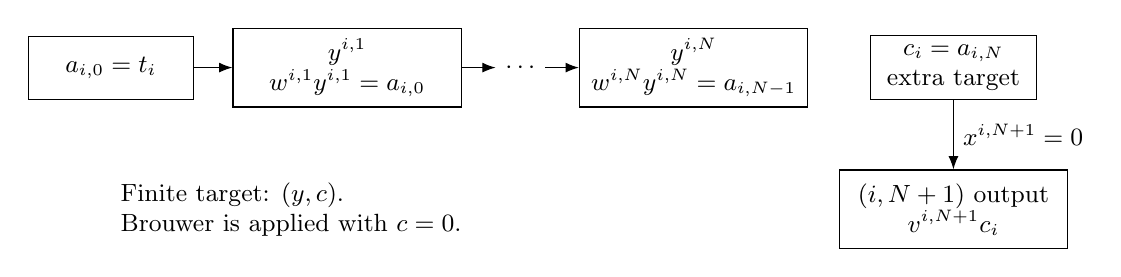
\begin{tikzpicture}[
  >=Latex,
  every node/.style={font=\small},
  block/.style={draw,minimum width=29mm,minimum height=10mm,align=center},
  scalar/.style={draw,minimum width=21mm,minimum height=8mm,align=center}
]
\node[scalar] (a0) at (0,0) {\(a_{i,0}=t_i\)};
\node[block] (y1) at (3.0,0) {\(y^{i,1}\)\\\(w^{i,1}y^{i,1}=a_{i,0}\)};
\node (dots) at (5.2,0) {\(\cdots\)};
\node[block] (yn) at (7.4,0) {\(y^{i,N}\)\\\(w^{i,N}y^{i,N}=a_{i,N-1}\)};
\node[scalar] (terminal) at (10.7,0) {\(c_i=a_{i,N}\)\\extra target};
\draw[->] (a0) -- (y1);
\draw[->] (y1) -- (dots);
\draw[->] (dots) -- (yn);
\node[block] (spill) at (10.7,-1.8)
 {\((i,N+1)\) output\\\(v^{i,N+1}c_i\)};
\draw[->] (terminal) -- node[right,align=left]
 {\(x^{i,N+1}=0\)} (spill);
\node[align=left,anchor=west] at (0,-1.8)
 {Finite target: \((y,c)\).\\
  Brouwer is applied with \(c=0\).};
\end{tikzpicture}
\caption{A row of length \(N\) with frozen weights and independent
extra target scalar \(c_i=a_{i,N}\). The block readouts recover the
predecessor scalars, while \(c_i\) records the scalar not read by any
block in the finite row. At the nonlinear
fixed point it is set to zero, which kills the only possible output
spillover into the next block.}
\label{fig:terminal}
\end{figure}


Let \(0\ne y\in U_N\), and set \(h=\|y\|_U>0\). On the closed ball
\(\{x\in D_N:\|x\|_D\leq5h\}\), define
\begin{equation}
 s(x)=\frac{x}{\max\{\|x\|_D,h/6\}},\qquad
 T(x)=(S_{s(x)}^{(N)})^{-1}(y,0).                            \label{eq:brouwer-map}
\end{equation}
The denominator is positive even at \(x=0\), so \(s(x)\in B\)
depends continuously on \(x\). Equations \eqref{eq:finite-inverse}--\eqref{eq:finite-bounds} show that \(T\)
is a continuous self-map of this finite-dimensional closed ball.
Brouwer's fixed-point theorem gives \(x=T(x)\). At that fixed point,
\[
       h=\|(y,0)\|=\|S_{s(x)}^{(N)}x\|\leq5\|x\|_D,
\]
and therefore \(\|x\|_D\geq h/5>h/6\). The state in \eqref{eq:brouwer-map} is now
the normalized state \(s_x\), not the regularized state used near zero.
The blocks of \(g(x)\) in the \(N\)-square are \(y\), and \eqref{eq:finite-shift} gives
\(a_{i,N}=0\) for every \(i\leq N\).

It remains to check the blocks omitted from the finite equation.
The input is zero outside \(D_N\). The only outside block with a
possibly nonzero predecessor scalar is \((i,N+1)\) for \(i\leq N\).
There
\[
 (g(x))^{i,N+1}
       =v^{i,N+1}(s_x)a_{i,N}=0.
\]
All other outside blocks have zero input and zero predecessor scalar.
Thus \(g(x)=y\) in \(U\). The zero target is \(g(0)\), so
\(U_N\subset g(D)\) for every \(N\).

Every finitely supported element of \(U\) belongs to some \(U_N\),
and such elements are dense. The image \(g(D)\) is closed: if
\(g(x_k)\) converges in \(U\), the positive lower bound \eqref{eq:global-bounds} makes
\((x_k)\) Cauchy in the Banach space \(D\); its limit \(x\) satisfies
\(g(x_k)\to g(x)\) by continuity. Hence \(g(D)\) is both dense and
closed in \(U\), and is all of \(U\).
\end{proof}

Let \(P:D\to U\) be the projection and, for \(s\in B\), put
\begin{equation}
                         h(s)=(S_s-P)s.                      \label{eq:h-definition}
\end{equation}
The frozen lemma ensures \(h(s)\in U\), and \eqref{eq:correction-coordinate} is exactly its
\(\gamma\)-coordinate. Notice that \(S_s s\) uses \(s\) itself
as state even when \(\|s\|<1\), whereas \(g(s)\) uses \(s/\|s\|\).
The lifting argument will use \eqref{eq:h-definition} on \(B\) and \eqref{eq:g-definition} only on
normalized states. By \eqref{eq:correction-bounds}, the correction coordinates have common
bounds
\begin{equation}
 A:=\sup_\gamma\|f_\gamma\|_\infty\leq4,\qquad
 L_0:=\sup_\gamma\Lip(f_\gamma)\leq4+12\eta.                  \label{eq:base-bounds}
\end{equation}

\section{Selected tests and their supports}\label{sec:tests}

The next goal is to construct a Banach space that lifts the correction
\(h(s)=(S_s-P)s\) and contains no linear \(c_0\). We use the coordinate
functions \(f_\gamma\) of \eqref{eq:correction-coordinate}, with exactly the finite-dependence and
support assertions \eqref{eq:correction-bounds}--\eqref{eq:correction-support}. The operations below enlarge the family
of tests while retaining quantitative control of where each test can
be nonzero.

\subsection{Two local operations}

Fix a label \(\gamma=(\lambda,j,\xi)\) and its nonempty finite set
\(I=I_\gamma\). A function on \(B\) depending only on \(I\) is
identified with its function on the cube \([-1,1]^I\), by evaluating
at the zero extension of a cube point. Write \(s|_I\) for coordinate
restriction. For a dyadic scale \(\varepsilon=2^{-a}\),
\(a\in\N_0=\{0,1,\ldots\}\), let
\[
 \mathcal Q_{I,\varepsilon}
   =\bigl([-1,1]\cap(\varepsilon/8)\mathbb Z\bigr)^I .
\]
This is a finite grid including both endpoints in each coordinate.
Every point of the cube is within \(\varepsilon/16\), hence within
\(\varepsilon/8\), of a grid point in the supremum norm.

Define the \(2\)-Lipschitz function
\[
 \chi(t)=
 \begin{cases}
 0,&0\leq t\leq1/2,\\
 2t-1,&1/2<t<1,\\
 1,&t\geq1.
 \end{cases}
\]
For a Lipschitz function \(u\) depending on \(I\), and
\(q\in\mathcal Q_{I,\varepsilon}\), put
\begin{align}
 (G_{q,\varepsilon}u)(s)
 &=u(q)+\chi\!\left(\frac{\|s|_I-q\|_\infty}{\varepsilon}\right)
                    (u(s)-u(q)), \label{eq:G}\\
 R_{q,\varepsilon}u&=G_{q,\varepsilon}u-u. \label{eq:R}
\end{align}
Here \(u(q)\) means evaluation at the zero extension of \(q\).
Both operations are linear in \(u\), retain dependence on \(I\), and
\(G_{q,\varepsilon}u\) is the constant \(u(q)\) on the open cylinder
\(\|s|_I-q\|_\infty<\varepsilon/2\).
Thus \(G\) makes \(u\) locally constant and changes it only inside
the radius-\(\varepsilon\) cylinder; \(R\) records that change.
The identity \(G=\mathrm{Id}+R\) will separate fixed parts of a test
from changes occurring at small scales.

\begin{lemma}[Bounds and geometric support]\label{lem:operations}
For every such \(u,q,\varepsilon\),
\begin{align}
 \|R_{q,\varepsilon}u\|_\infty
   &\leq\varepsilon\Lip(u),&
 \Lip(R_{q,\varepsilon}u)&\leq3\Lip(u),&
 \Lip(G_{q,\varepsilon}u)&\leq4\Lip(u), \label{eq:operation-lip}\\
 \|G_{q,\varepsilon}u\|_\infty
   &\leq\|u\|_\infty,&
 \|R_{q,\varepsilon}u\|_\infty&\leq2\|u\|_\infty. \label{eq:operation-sup}
\end{align}
Let
\[
 K_I(u)=\overline{\{s|_I:s\in B,\ u(s)\ne0\}}^{\,[-1,1]^I}.
\]
In the next display write \(G=G_{q,\varepsilon}\) and
\(R=R_{q,\varepsilon}\).
With \(K_\varepsilon=\{p:\operatorname{dist}_\infty(p,K)\leq
\varepsilon\}\) and \(\varnothing_\varepsilon=\varnothing\), one has
\begin{equation}
 K_I(Gu),K_I(Ru)\subset K_I(u)_\varepsilon,\qquad
 K_I(Ru)\subset\overline B_\infty(q,\varepsilon).             \label{eq:operation-support}
\end{equation}
\end{lemma}

\begin{proof}
Set \(a(s)=1-\chi(\|s|_I-q\|_\infty/\varepsilon)\). Then
\[
 R_{q,\varepsilon}u(s)=a(s)(u(q)-u(s)),\qquad
 0\leq a\leq1,\qquad \Lip(a)\leq2/\varepsilon.
\]
If \(a(s)\ne0\), then \(\|s|_I-q\|_\infty<\varepsilon\);
the cylindrical Lipschitz bound gives
\(|u(q)-u(s)|\leq\varepsilon\Lip(u)\). This proves the first
supremum estimate in \eqref{eq:operation-lip}.

To compare \(Ru(s)\) and \(Ru(t)\), there is nothing to prove if both
values of \(a\) are zero. Otherwise interchange \(s,t\), if needed,
so that \(a(t)\ne0\). The identity
\[
 Ru(s)-Ru(t)
 =a(s)(u(t)-u(s))+(a(s)-a(t))(u(q)-u(t))
\]
bounds the two terms by \(\Lip(u)\|s-t\|_D\) and
\((2/\varepsilon)\|s-t\|_D\,\varepsilon\Lip(u)\), respectively.
Thus \(\Lip(Ru)\leq3\Lip(u)\), and \(Gu=u+Ru\) gives
\(\Lip(Gu)\leq4\Lip(u)\). The formula for \(G\) is a convex
combination of \(u(q)\) and \(u(s)\), so it does not increase the
supremum norm. The bound for \(R=G-u\) follows.

For the support assertions, if a new output is nonzero at \(s\) while
\(u(s)=0\), then \(u(q)\ne0\) and
\(\|s|_I-q\|_\infty<\varepsilon\). If \(u(s)\ne0\), its projection
already lies in \(K_I(u)\). This covers both \(G\) and \(R\).
Taking closures gives their inclusion in \(K_I(u)_\varepsilon\);
the latter set is closed because the cube is compact. In addition,
\(Ru(s)=0\) whenever \(\|s|_I-q\|_\infty\geq\varepsilon\),
which proves its ball inclusion. If \(u=0\), all statements are
immediate.
\end{proof}

\subsection{Scale budgets and tail factors}

For \(h\geq1\), let \(\mathcal T_h\) consist of functions obtained
from a single \(f_\gamma\), \(\gamma=(\lambda,j,\xi)\), by \(m\leq h\)
successive operations \(G\) or \(R\) on \(I_\gamma\). A representation
with \(m=0\) is allowed. For \(m\geq1\), the scales in their order of
application must satisfy
\begin{equation}
 \varepsilon_1\geq\varepsilon_2\geq\cdots\geq\varepsilon_m>0,
 \qquad
 \sum_{k=1}^m\varepsilon_k<\frac{\ell_j}{2}.                 \label{eq:scale-rule}
\end{equation}
The sum is zero for \(m=0\). Each scale is dyadic and each center is
in its corresponding finite grid. We refer to \(\gamma\) as a
representing label, since a function may have more than one
representation. The strict inequality leaves a positive amount of
budget for a further sufficiently small operation. The order will
ensure that every operation after a small one has at most that scale.

For a continuous function on \(B\), let
\(\supp_B u=\overline{\{s\in B:u(s)\ne0\}}^{\,B}\).
All support statements refer to these concrete generated functions.
Later, molecule pairings will ignore additive constants, but we do not
replace a generated function by another representative modulo constants:
that could change its support and its constant value on a cylinder.

\begin{lemma}[Propagation of the correction support]\label{lem:support}
Suppose \(u\in\mathcal T_h\) has a representation based at
\(\gamma=(\lambda,j,\xi)\) with total scale
\(e=\sum_{k=1}^m\varepsilon_k\). On \(\supp_B u\),
\begin{equation}
 \begin{cases}
 \|\pi_j s-\xi\|_\infty\leq2d_j+e,&j\geq1,\\
 r_\lambda(s)\geq\ell_j-e,&j<J_\lambda.
 \end{cases}                                                  \label{eq:support-sharp}
\end{equation}
In particular, on the same support,
\begin{equation}
 \begin{cases}
 \|\pi_j s-\xi\|_\infty\leq2d_j+\ell_j/2,&j\geq1,\\
 r_\lambda(s)\geq\ell_j/2,&j<J_\lambda.
 \end{cases}                                                  \label{eq:support-coarse}
\end{equation}
\end{lemma}

\begin{proof}
Start with \eqref{eq:correction-support}, which holds on the relative support of \(f_\gamma\)
as well as its nonzero set, because its two inequalities describe
closed subsets of \(B\). Suppose the claim has been proved for the
old function and add an operation of scale \(\varepsilon\).
If the new function is nonzero at \(s\) and the old one is zero there,
the proof of Lemma~\ref{lem:operations} gives an old nonzero value
at the zero extension of \(q\), with
\(\|s|_{I_\gamma}-q\|_\infty<\varepsilon\). Otherwise the old
support already contains \(s\). Both \(\pi_j\) and \(r_\lambda\)
depend only on \(I_\gamma\); coordinate restriction has norm one,
and \(r_\lambda\) is \(1\)-Lipschitz on that cube. The first upper
bound therefore increases by at most \(\varepsilon\), and the
second lower bound decreases by at most \(\varepsilon\).
Induction proves \eqref{eq:support-sharp} on the nonzero set.
Taking relative closure preserves the closed inequalities. Finally,
\eqref{eq:scale-rule} gives \eqref{eq:support-coarse}.
\end{proof}

For \(N\geq1\), define the coordinate tail
\begin{equation}
 \tau_N(s)=\sup_{k>N}|s_k|,\qquad
 b_{c,N}(s)=\min\{1,(2-\tau_N(s)/c)_+\}\quad(c>0),
                                                               \label{eq:tail}
\end{equation}
where \(a_+=\max\{a,0\}\). The function \(\tau_N\) is
\(1\)-Lipschitz, and \(\tau_N(s)\to0\) for each \(s\in B\).
Both \(b_{c,N}\) and \(b_{c,N}-1\) have supremum norm at most one
and Lipschitz constant at most \(1/c\). Their relative supports satisfy
\begin{equation}
 \supp_B b_{c,N}\subset\{\tau_N\leq2c\},\qquad
 \supp_B(b_{c,N}-1)\subset\{\tau_N\geq c\}.                  \label{eq:tail-support}
\end{equation}
For example, the first function vanishes when \(\tau_N\geq2c\),
and the second vanishes when \(\tau_N\leq c\); closure gives the
displayed weak inequalities.

Let \(\mathcal V_h\) consist of all products
\begin{equation}
                         u\prod_{r=1}^l\beta_r              \label{eq:Vclass}
\end{equation}
where \(u\in\mathcal T_h\) has a representing label with \(j\leq h\),
\(0\leq l\leq h\), and each \(\beta_r\) is \(b_{c_r,N_r}\) or
\(b_{c_r,N_r}-1\), with \(N_r\geq1\) and
\[
                       c_r\in\{2^{-a}:0\leq a\leq h\}.
\]
The empty product is one. The support of a product is contained in
the support of its cylindrical factor \(u\), so every such test
inherits \eqref{eq:support-coarse}. We will use the countable list of
classes
\begin{equation}
               \mathcal T_1,\mathcal V_1,
               \mathcal T_2,\mathcal V_2,\ldots.             \label{eq:classes}
\end{equation}

\begin{lemma}[Bounds in each fixed class]\label{lem:class-bounds}
With \(A,L_0\) from \eqref{eq:base-bounds}, the following bounds are uniform over all
tests of the indicated class:
\begin{equation}
 \begin{array}{c|cc}
 &\|u\|_\infty&\Lip(u)\\ \hline
 u\in\mathcal T_h&2^hA&4^hL_0\\
 u\in\mathcal V_h&2^hA&4^hL_0+h4^hA.
 \end{array}                                                  \label{eq:class-bounds}
\end{equation}
\end{lemma}

\begin{proof}
Iterating \eqref{eq:operation-lip}--\eqref{eq:operation-sup}
gives the first row. For the second, every tail factor has supremum
norm at most one and Lipschitz constant at most \(2^h\). A product
of at most \(h\) such factors has Lipschitz constant at most
\(h2^h\), by telescoping the product difference. The product rule
then gives
\[
 \Lip\!\left(u\prod_r\beta_r\right)
 \leq4^hL_0+(2^hA)(h2^h)=4^hL_0+h4^hA.
\]
Its supremum norm is at most \(2^hA\).
\end{proof}

We have two useful consequences of the support bounds. For a fixed
bounded set of bands \(j\), the second line of
\eqref{eq:support-coarse} gives a positive radial threshold whenever
\(j<J_\lambda\). For \(j\to\infty\), the first line confines the
first \(j\) coordinates to a radius
\(2d_j+\ell_j/2\to0\). Section~\ref{sec:no-c0} will use precisely
these alternatives, after the next section extends the tests from
finite molecules to the completed Banach space.

\section{Molecules and the lifted correction}\label{sec:molecules}

We now turn the selected tests into a Banach space. The norm must do
two jobs: control point differences so that the correction can be
lifted Lipschitzly, and remember lists of tests whose signed sums have
a common Lipschitz bound. The latter feature will rule out linear
\(c_0\).

\subsection{The quotient and its completion}

Let \(\mathcal M_0(B)\) be the real vector space of mass-zero finite
formal sums
\[
 m=\sum_{s\in B}a_s\delta_s,\qquad
 \#\{s:a_s\ne0\}<\infty,\qquad \sum_s a_s=0.
\]
For a real function \(u\) on \(B\), set
\(\langle u,m\rangle=\sum_s a_su(s)\). Constants pair to zero.
This follows the mass-zero molecule construction of Arens and Eells
\cite{AE56} and its later Lipschitz-free formulation \cite{GK03}.
The norm below is built from the selected classes
\eqref{eq:classes}; no universal property of the usual free space is
assumed.

For every triple \(d=(\mathcal L,C,p)\), where \(\mathcal L\) is one
of the listed classes, \(C\in\N\), and \(p=1+1/k\) for \(k\in\N\),
define
\begin{equation}
 \sigma_d(m)=
 \sup\left\{
 \left(\sum_{\nu=1}^l|\langle u_\nu,m\rangle|^p\right)^{1/p}:
 \begin{array}{l}
 l\geq0,\quad u_1,\ldots,u_l\in\mathcal L,\\
 \Lip\!\left(\sum_{\nu=1}^l e_\nu u_\nu\right)\leq C
 \ \text{for every }(e_\nu)\in\{-1,1\}^l
 \end{array}\right\}.                                      \label{eq:sigma}
\end{equation}
The empty list contributes zero. Lists may contain repetitions and
tests with the same representing label; their sole compatibility
condition is the displayed Lipschitz bound for every choice of signs.
Equivalently, a list is admissible precisely when
\begin{equation}
 \sum_{\nu=1}^l|u_\nu(s)-u_\nu(t)|\leq C\|s-t\|_D
                   \qquad(s,t\in B).
 \label{eq:admissible-increments}
\end{equation}
To obtain this inequality, choose signs matching the increments
\(u_\nu(s)-u_\nu(t)\); the converse follows from the triangle inequality.

Enumerate the triples by \(d=1,2,\ldots\), write \(C_d\) for their
integer component, and set
\begin{equation}
             \alpha_d=\frac{2^{-d}}{C_d^2},\qquad
 \|m\|_0=\left(\sum_{d\geq1}\alpha_d\sigma_d(m)^2\right)^{1/2}.
                                                               \label{eq:norm}
\end{equation}

The outer square sum and the exponents approaching one serve distinct
purposes in Section~\ref{sec:no-c0}. The square sum forces one fixed
seminorm to detect a subsequence of any hypothetical \(c_0\) basis.
For that fixed test class and Lipschitz bound, a second exponent
\(p'<p\) converts detection by a list into detection by one scalar
test. Both choices are part
of the obstruction, as well as of the norm construction.

\begin{lemma}[Exact completed norm]\label{lem:completion}
Formula \eqref{eq:norm} is a finite seminorm on \(\mathcal M_0(B)\).
Let \(N\) be its kernel, and let \(Z\) be the Banach completion of
\(\mathcal M_0(B)/N\) with the induced norm. Then \(Z\) is separable,
and
\begin{equation}
 \zeta:B\to Z,\qquad \zeta(s)=[\delta_s-\delta_0]             \label{eq:zeta}
\end{equation}
is \(1\)-Lipschitz with \(\zeta(0)=0\). Each \(\sigma_d\) descends
and extends continuously to a seminorm on \(Z\), and the exact formula
\begin{equation}
                    \|z\|_Z^2=\sum_{d\geq1}
                                \alpha_d\sigma_d(z)^2         \label{eq:completed-norm}
\end{equation}
holds for every \(z\in Z\).
\end{lemma}

\begin{proof}
For \(s,t\in B\) and an admissible list for \(d\), inequality
\eqref{eq:admissible-increments} bounds the sum of the absolute
increments. Since the \(\ell_p\) norm is no larger than this sum,
\begin{equation}
                 \sigma_d(\delta_s-\delta_t)
                         \leq C_d\|s-t\|_D.                  \label{eq:molecule-bound}
\end{equation}
For a fixed list, Minkowski's inequality makes its expression in
\eqref{eq:sigma} a seminorm in \(m\); the supremum of these expressions
is also a seminorm, once finite. Every \(m=\sum_s a_s\delta_s\)
of mass zero equals \(\sum_s a_s(\delta_s-\delta_0)\). Thus
\[
 \sigma_d(m)\leq C_d\sum_s|a_s|\|s\|_D.
\]
This proves finiteness both of \(\sigma_d\) and of \(\|m\|_0\),
because \(\sum_d\alpha_d C_d^2=\sum_d2^{-d}=1\).
Minkowski's inequality in \(\ell_2\), applied to the weighted
seminorms, proves subadditivity of \(\|\cdot\|_0\); homogeneity is
immediate. Its kernel is therefore a linear subspace, and quotienting
by it produces a norm.

Equation \eqref{eq:molecule-bound} and the same square sum give
\[
                   \|\delta_s-\delta_t\|_0\leq\|s-t\|_D.
\]
This proves the assertion about \(\zeta\). The ball \(B\) is separable
because \(D\) is a countable-coordinate \(c_0\) space. If \(B_0\) is
a countable dense subset, continuity of \(\zeta\) makes
\(\zeta(B_0)\) dense in \(\zeta(B)\). The real linear span of
\(\zeta(B)\) is the quotient molecule space; its rational span over
\(B_0\) is consequently dense in \(Z\). Hence \(Z\) is separable.

For molecules \(m,m'\),
\begin{equation}
 |\sigma_d(m)-\sigma_d(m')|
 \leq\sigma_d(m-m')\leq\alpha_d^{-1/2}\|m-m'\|_0.            \label{eq:sigma-continuity}
\end{equation}
In particular \(\sigma_d\) vanishes on \(N\), descends, and extends
continuously to \(Z\); subadditivity and homogeneity pass to limits.
Moreover the map
\[
 m\longmapsto(\sqrt{\alpha_d}\sigma_d(m))_{d\geq1}
\]
is \(1\)-Lipschitz into \(\ell_2\), since the coordinate differences
are bounded by \(\sqrt{\alpha_d}\sigma_d(m-m')\). If molecules
converge to \(z\in Z\), their images therefore converge in \(\ell_2\).
The \(d\)-th coordinate of the limit is
\(\sqrt{\alpha_d}\sigma_d(z)\) by continuity of each seminorm.
The norms of those images are exactly the molecule norms, which
converge to \(\|z\|_Z\). This proves \eqref{eq:completed-norm}.
\end{proof}

\subsection{Fixed-class duality}

The obstruction argument will modify a test through a pointwise
limit after a vector in \(Z\) has already been fixed. The next lemma
justifies that passage, and also retains the exact list formula after
completion.

\begin{lemma}[Dual tests and pointwise limits]\label{lem:duality}
Every test in \(\mathcal T_h\) or \(\mathcal V_h\) defines a bounded
linear functional on \(Z\) by its molecule pairing. For each fixed
class \(\mathcal L\), there is a finite common bound \(B_{\mathcal L}\)
for these dual norms. For each fixed triple \(d=(\mathcal L,C,p)\),
formula \eqref{eq:sigma} remains exact on \(Z\), with the extended
test pairings.

If \(u_n\in\mathcal L\) and \(u_n(s)\to u(s)\) for every \(s\in B\),
then the pointwise limit defines a bounded functional on \(Z\) of
norm at most \(B_{\mathcal L}\), and
\(\langle u_n,z\rangle\to\langle u,z\rangle\) for each fixed
\(z\in Z\). More precisely, for any molecule class \(m\) and any
\(z\in Z\),
\begin{equation}
 |\langle u_n-u,z\rangle|
 \leq|\langle u_n-u,m\rangle|
       +2B_{\mathcal L}\|z-m\|_Z.                            \label{eq:fixed-vector}
\end{equation}
\end{lemma}

\begin{proof}
Choose an integer \(C_{\mathcal L}\) no smaller than the uniform
Lipschitz bound in Lemma~\ref{lem:class-bounds}. Every singleton
\((u)\), \(u\in\mathcal L\), is admissible for the one triple
\(d_{\mathcal L}=(\mathcal L,C_{\mathcal L},2)\). Thus
\begin{equation}
 |\langle u,m\rangle|
 \leq\sigma_{d_{\mathcal L}}(m)
 \leq\alpha_{d_{\mathcal L}}^{-1/2}\|m\|_0.                 \label{eq:dual-bound}
\end{equation}
It vanishes on \(N\) and extends to \(Z^*\), uniformly with
\(B_{\mathcal L}=\alpha_{d_{\mathcal L}}^{-1/2}\).

For an admissible list \(\boldsymbol u=(u_1,\ldots,u_l)\) of a
fixed triple \(d\), its evaluation map
\(\Lambda_{\boldsymbol u}m=(\langle u_\nu,m\rangle)_{\nu=1}^l\)
into \(\ell_p^l\) has norm at most \(\alpha_d^{-1/2}\) on the
molecule quotient. It therefore extends with that bound to \(Z\).
The supremum of \(\|\Lambda_{\boldsymbol u}z\|_p\) over all admissible
lists is finite and \(\alpha_d^{-1/2}\)-Lipschitz as a seminorm in
\(z\): its change between \(z,z'\) is bounded by the same supremum
at \(z-z'\). This supremum agrees with \(\sigma_d\) on the dense
molecule quotient. It is therefore the continuous extension of
\(\sigma_d\), which proves the exact formula on \(Z\).

For a pointwise-convergent sequence, the pairings converge on every
finite molecule. Inequality \eqref{eq:dual-bound} passes to that
pointwise limit, so its molecule functional extends with norm at most
\(B_{\mathcal L}\). Applying the two common dual bounds to \(z-m\)
gives \eqref{eq:fixed-vector}. For a prescribed \(z\) and tolerance
\(\delta>0\), choose a molecule class \(m\) with
\(\|z-m\|_Z<\delta/(4B_{\mathcal L})\), and then choose \(n\) so large
that the finite pairing in \eqref{eq:fixed-vector} is less than
\(\delta/2\). This proves convergence on \(z\). The choice of \(m\)
and \(n\) may depend on \(z\); no convergence uniform over a moving
sequence of vectors is asserted.
\end{proof}

\begin{lemma}[The \(c_0\)-valued correction map]\label{lem:Q}
There is a bounded linear map \(Q:Z\to U\) such that
\begin{equation}
                         Q\zeta(s)=h(s)=(S_s-P)s
                         \qquad(s\in B).                    \label{eq:Qzeta}
\end{equation}
\end{lemma}

\begin{proof}
Define on formal molecules
\[
                  Q_0m=\sum_s a_s h(s)\in U.
\]
This finite sum lies in \(U\), not merely in \(\ell_\infty\), because
each \(h(s)\) lies in \(U\). Each coordinate function \(f_\gamma\)
belongs to \(\mathcal T_1\) through its zero-operation representation.
Choose an integer \(C_0\geq L_0\) and the triple
\(d_0=(\mathcal T_1,C_0,2)\). Every singleton \((f_\gamma)\) is
admissible, whence
\[
 \|Q_0m\|_U=\sup_\gamma|\langle f_\gamma,m\rangle|
 \leq\sigma_{d_0}(m)\leq\alpha_{d_0}^{-1/2}\|m\|_0.
\]
Thus \(Q_0\) vanishes on \(N\), descends, and extends to a bounded
linear map into the complete space \(U\). Since \(h(0)=0\), applying
it to \(\delta_s-\delta_0\) proves \eqref{eq:Qzeta}.
\end{proof}

\subsection{Radial extension}

The point map \(\zeta\) is defined on \(B\). Its radial extension
lifts the homogeneous shift correction on all of \(D\).

\begin{lemma}[Lipschitz lift]\label{lem:K}
Define
\begin{equation}
 K(0)=0,\qquad
 K(x)=\|x\|_D\,\zeta\!\left(\frac{x}{\|x\|_D}\right)
                         \quad(x\ne0).                       \label{eq:K}
\end{equation}
Then \(K:D\to Z\) is positively homogeneous and
\(\Lip(K)\leq3\). It satisfies the exact identity
\begin{equation}
                              QK=g-P.                        \label{eq:lift}
\end{equation}
\end{lemma}

\begin{proof}
Since \(\zeta(0)=0\) and \(\Lip(\zeta)\leq1\),
\(\|\zeta(s)\|_Z\leq1\) for \(s\in B\). Suppose
\(a=\|x\|_D\geq b=\|x'\|_D>0\), and write \(s=x/a\), \(s'=x'/b\).
Splitting at \(b\zeta(s)\) gives
\[
 \|K(x)-K(x')\|_Z
 \leq(a-b)\|\zeta(s)\|_Z+b\|\zeta(s)-\zeta(s')\|_Z
 \leq\|x-x'\|_D+b\|s-s'\|_D.
\]
The normalization estimate \eqref{eq:normalization} bounds the last term by
\(2\|x-x'\|_D\). If an endpoint is zero, use
\(\|K(x)\|_Z\leq\|x\|_D\). This proves the Lipschitz bound.
For \(x\ne0\), \eqref{eq:Qzeta}, \eqref{eq:h-definition}, and \eqref{eq:g-definition} give
\[
 QK(x)=\|x\|_D h(x/\|x\|_D)
      =S_{x/\|x\|_D}x-Px=g(x)-Px.
\]
All terms vanish at zero, and positive homogeneity follows directly
from \eqref{eq:K}.
\end{proof}

We have now obtained the exact data \(Q,K,g\) of
Lemma~\ref{lem:absorption}. No surjectivity of \(Q\) was used or
proved. The remaining task is to show that the completed space \(Z\)
has no linear copy of \(c_0\).

\section{Detectors exclude linear \texorpdfstring{\(c_0\)}{c0}}\label{sec:no-c0}

A linear copy of \(c_0\) would provide vectors bounded away from zero
whose finite signed sums are uniformly bounded. We first show that
one class of tests detects a subsequence of these vectors. We then
identify the additional property needed for a contradiction: the tests'
finite signed sums must have one Lipschitz bound. The rest of the
section obtains this property by modifying the detectors and separating
or nesting their supports. Supports always refer to the concrete
generated functions on \(B\).

\subsection{From bounded signed sums to individual detectors}

The extraction has two stages. The outer square sum prevents detection
from escaping through different seminorms; within one seminorm, the
exponents approaching one prevent it from spreading over arbitrarily
many small scalar pairings.

\begin{lemma}[One class detects a subsequence]\label{lem:detectors}
Suppose \((m_i)\subset Z\) satisfies, for some \(r,M>0\),
\begin{equation}
 \|m_i\|_Z\geq r,\qquad
 \left\|\sum_{i\in H}\epsilon_i m_i\right\|_Z\leq M
 \quad\text{for all finite \(H\) and all signs \(\epsilon_i\)}. \label{eq:bounded-signed}
\end{equation}
Then \(u(m_i)\to0\) for every \(u\in Z^*\). After a subsequence,
there are tests \(F_i\) in one listed class \(\mathcal L\) and a
constant \(\delta>0\) with
\begin{equation}
                         |\langle F_i,m_i\rangle|\geq\delta.
                                                               \label{eq:detected}
\end{equation}
\end{lemma}

\begin{proof}
For any fixed \(u\in Z^*\), choosing signs matching \(u(m_i)\) in
\eqref{eq:bounded-signed} gives
\[
                    \sum_{i\in H}|u(m_i)|\leq M\|u\|
\]
for every finite \(H\). Thus \(\sum_i|u(m_i)|<\infty\), and in
particular \(u(m_i)\to0\). Also \(\|m_i\|\leq M\).

We first prove that one fixed seminorm stays away from zero on a
subsequence. Otherwise \(\sigma_d(m_i)\to0\) for every \(d\).
The vectors
\[
               v_i=(\sqrt{\alpha_d}\sigma_d(m_i))_{d\geq1}
\]
then converge coordinatewise to zero in \(\ell_2\), while
\(r\leq\|v_i\|_2=\|m_i\|_Z\leq M\). A direct gliding-hump selection
gives disjoint finite intervals \(A_i\) of indices, after a
subsequence, such that
\begin{equation}
                 \sum_{d\in A_i}\alpha_d\sigma_d(m_i)^2
                            \geq r^2/4.                      \label{eq:hump-mass}
\end{equation}
Indeed, once the endpoint of the preceding interval is fixed,
coordinatewise convergence makes the squared mass before that
endpoint less than \(r^2/4\) for a sufficiently late \(v_i\).
Then choose a new finite endpoint so that the squared tail mass is
less than \(r^2/4\). The mass in between is at least \(r^2/2\),
which implies \eqref{eq:hump-mass}.

The function \(\sigma_d^2\) is even and convex, because a seminorm
is convex and squaring is convex and increasing on \([0,\infty)\).
For fixed \(y,m\),
Jensen's inequality applied to \(y+m\) and \(-y+m\) gives
\begin{equation}
       \frac{\sigma_d(y+m)^2+\sigma_d(y-m)^2}{2}
                        \geq\sigma_d(m)^2.                  \label{eq:seminorm-convexity}
\end{equation}
For independent random signs and a finite \(H\), average first over
the sign of \(m_i\) and use \eqref{eq:seminorm-convexity}. Thus
\[
 \mathbb E\,\sigma_d\!\left(\sum_{k\in H}\epsilon_km_k\right)^2
                         \geq\sigma_d(m_i)^2\quad(i\in H).
\]
The exact norm formula, \eqref{eq:bounded-signed}, the disjointness of the \(A_i\), and
\eqref{eq:hump-mass} imply
\[
 M^2\geq\mathbb E\left\|\sum_{k\in H}\epsilon_km_k\right\|_Z^2
 \geq\sum_{i\in H}\sum_{d\in A_i}\alpha_d\sigma_d(m_i)^2
 \geq |H|r^2/4,
\]
a contradiction for large \(H\). Hence some
\(d=(\mathcal L,C,p)\) has \(\sigma_d(m_i)\geq a>0\) on a subsequence.

Choose a listed exponent \(p'=1+1/k'<p\), with the same
\(\mathcal L,C\), and call its triple \(d'\). Its seminorm is bounded
on these vectors by
\[
                  \sigma_{d'}(m_i)\leq
                  \alpha_{d'}^{-1/2}M=:B_0.
\]
For each \(i\), choose a finite admissible list for \(d\) whose
\(\ell_p\) value on \(m_i\) is at least \(a/2\). Put
\(x_\nu=|\langle u_\nu,m_i\rangle|\). The same list is admissible
for \(d'\), because only the exponent changed. Consequently
\[
 (a/2)^p\leq\sum_\nu x_\nu^p
 \leq(\max_\nu x_\nu)^{p-p'}\sum_\nu x_\nu^{p'}
 \leq(\max_\nu x_\nu)^{p-p'}B_0^{p'}.
\]
The list is nonempty and \(B_0>0\). One of its tests therefore has
evaluation at least
\[
             \delta=\left(\frac{(a/2)^p}{B_0^{p'}}\right)^{1/(p-p')}>0.
\]
Choosing that test as \(F_i\) proves \eqref{eq:detected}.
\end{proof}

\subsection{The growth forced by compatible detectors}

Call a sequence of tests \emph{compatible} if all its finite signed
sums have a common Lipschitz bound. The norm was defined using precisely
such lists. Once compatible tests detect the vectors, a single
seminorm forces the following growth.

\begin{lemma}[Growth from compatible detectors]\label{lem:detector-growth}
Let \((m_i)\subset Z\), and let \(F_i\) belong to one listed class
\(\mathcal L\). Suppose there are \(\delta>0\) and an integer
\(C\geq1\) such that
\[
 |\langle F_i,m_i\rangle|\geq\delta,
 \qquad
 \Lip\!\left(\sum_{i\in H}\epsilon_iF_i\right)\leq C
\]
for every \(i\), every finite \(H\), and all signs \(\epsilon_i\).
For the listed triple \(d=(\mathcal L,C,2)\), every nonempty finite
\(H\) satisfies
\begin{equation}
 \max_{\epsilon_i\in\{-1,1\}}
 \left\|\sum_{i\in H}\epsilon_i m_i\right\|_Z
 \geq\sqrt{\alpha_d}\,\delta\sqrt{|H|}.
 \label{eq:detector-growth}
\end{equation}
\end{lemma}

\begin{proof}
The list \((F_k)_{k\in H}\) is admissible for \(d\), including when
labels repeat. For independent real random signs, the exact list
formula in Lemma~\ref{lem:duality} gives
\begin{align*}
 \mathbb E\,\sigma_d\!\left(\sum_{i\in H}\epsilon_i m_i\right)^2
 &\geq
 \mathbb E\sum_{k\in H}
       \left|\sum_{i\in H}\epsilon_i
                    \langle F_k,m_i\rangle\right|^2\\
 &=\sum_{k\in H}\sum_{i\in H}|\langle F_k,m_i\rangle|^2
 \geq |H|\delta^2.
\end{align*}
The equality uses cancellation of cross terms under the independent
signs; no cross-pairing is assumed to vanish. By
\eqref{eq:completed-norm},
\[
 \max_{\epsilon_i\in\{-1,1\}}
       \left\|\sum_{i\in H}\epsilon_i m_i\right\|_Z^2
 \geq\mathbb E\left\|\sum_{i\in H}\epsilon_i m_i\right\|_Z^2
 \geq\alpha_d|H|\delta^2.
\]
Taking square roots proves \eqref{eq:detector-growth}.
\end{proof}

It remains to make the detectors from Lemma~\ref{lem:detectors}
compatible without losing their nonzero pairings. We will use two
support configurations: disjoint supports, or later supports contained
in cylinders where earlier functions are constant.

\subsection{Support conditions for compatibility}

Localizing detecting Lipschitz functions and combining them with a
common Lipschitz bound is also central to Kalton's arguments for
metric free spaces \cite[Lemma~4.5 and proof of Theorem~4.6]{Kalton04}.
Here the supports are finite-coordinate cylinders and tail regions,
and their compatibility must be retained within the selected test
classes defining \(Z\).

\begin{lemma}[Compatible supports]\label{lem:compatible}
Let \(B\) be a convex subset of a normed space. Let \(u_i,b_i\)
be continuous real functions on \(B\), with \(b_i\) Lipschitz, and
put \(F_i=u_i b_i\). Suppose
\(\Lip(F_i)\leq L\) for every \(i\).
\begin{enumerate}
\item If the closed relative supports \(\supp_B F_i\) are pairwise
disjoint, every finite signed sum of the \(F_i\) has Lipschitz
constant at most \(L\).
\item Suppose that for each \(i\) there is a relatively open set
\(C_i\subset B\) and a scalar \(e_i\) such that \(u_i=e_i\) on
\(C_i\) and \(\supp_B u_k\subset C_i\) for every \(k>i\).
If \(\sum_i|e_i|\Lip(b_i)<\infty\), every finite signed sum of the
\(F_i\) has Lipschitz constant at most
\[
                         L+\sum_i|e_i|\Lip(b_i).
\]
If \(b_i=1\) for every \(i\), the summability condition is automatic.
\end{enumerate}
\end{lemma}

\begin{proof}
Fix a finite set of indices and signs. In the first case, at a given
point at most one of the corresponding closed supports contains that
point. All other summands vanish on a relative neighborhood, so the
sum is locally either zero or a single signed \(F_i\), with bound
\(L\).

In the second case, choose at a given point the largest selected
index \(j\) whose \(u_j\)-support contains the point. If there is no
such index, every summand vanishes on a common neighborhood, because
there are only finitely many closed supports. Otherwise all selected
later functions vanish on a neighborhood. The point lies in \(C_i\)
for each selected \(i<j\), so on a smaller neighborhood all those
\(u_i\) equal \(e_i\). On that neighborhood the sum is
\[
                \epsilon_jF_j+\sum_{\substack{i<j\\i\text{ selected}}}
                                  \epsilon_i e_i b_i,
\]
and has the asserted local Lipschitz bound.

To pass from the uniform local bound to a global bound, take any two
points of \(B\). The segment between them is contained in \(B\).
Its compact parameter interval has a finite cover by the relative
neighborhoods just obtained and hence a Lebesgue number. Subdivide
the segment finely enough that each subsegment lies in one such
neighborhood, apply the local estimate to each subsegment, and add.
The lengths of the collinear subsegments sum to the distance of the
endpoints. This proves both global assertions.
\end{proof}

\begin{lemma}[Tail separation]\label{lem:tail-separation}
Suppose \(F_i\) belong to one listed class and have representations
with bounded band indices. Suppose \(m_i\in Z\) and
\begin{equation}
 |\langle F_i,m_i\rangle|\geq\delta>0,\qquad
\supp_B F_i\subset\{\tau_{M_i}\geq c_*\},
 \quad M_i\in\N,\quad M_i\to\infty,\quad c_*>0.             \label{eq:tail-hypotheses}
\end{equation}
Then a subsequence has modified tests in one class \(\mathcal V_H\),
with detection at least \(\delta/2\), whose relative supports are
pairwise disjoint.
\end{lemma}

\begin{proof}
Choose a dyadic \(c=2^{-a}\) with \(2c<c_*\). If the original class
is \(\mathcal T_h\), view a test as a cylindrical factor with no tail
factors; if it is \(\mathcal V_h\), keep its chosen product
representation. A single integer \(H\), larger than \(h\), the
bounded band indices, and \(a\), can be chosen so that both \(F_i\)
and \(F_i b_{c,N}\) belong to \(\mathcal V_H\) for all \(i,N\).
There is room for one extra tail factor.

For each fixed \(i\), \(b_{c,N}(s)\to1\) at every \(s\in B\), since
\(\tau_N(s)\to0\). Lemma~\ref{lem:duality}, used in this one class,
therefore gives
\(\langle F_i b_{c,N},m_i\rangle\to\langle F_i,m_i\rangle\).
Choose \(N\) large enough that the difference has modulus less than
\(\delta/2\); every sufficiently large \(N\) then works. This choice
is made for the fixed vector \(m_i\).

Select indices recursively. After choosing an index \(i\) and such
an \(N_i\), take the next original index so far out that its \(M_k\)
exceeds all previously selected \(N_i\), which is possible because
\(M_k\to\infty\). Then choose its own \(N_k\) as above. For selected
\(k>i\), the new \(i\)-th support requires \(\tau_{N_i}\leq2c\)
by \eqref{eq:tail-support}. The new \(k\)-th support requires
\(\tau_{M_k}\geq c_*\) by \eqref{eq:tail-hypotheses}, hence
\(\tau_{N_i}\geq\tau_{M_k}\geq c_*>2c\). The supports are disjoint,
and the detection bound follows from the choice of \(N_i\).
\end{proof}

\subsection{Selecting compatible detectors}

The next proposition isolates the geometric part of the argument. It
uses only weak nullity of the vectors, one fixed test class, and a
uniform lower bound on the pairings. The bounded signed sums will enter
again only when we apply Lemma~\ref{lem:detector-growth}.

\begin{proposition}[Selection of compatible detectors]
\label{prop:compatible-detectors}
Let \((m_i)\subset Z\) be weakly null, meaning
\(u(m_i)\to0\) for every \(u\in Z^*\). Suppose \(F_i\) belong to one
listed class \(\mathcal L\) and
\begin{equation}
                  |\langle F_i,m_i\rangle|\geq\delta>0
                  \qquad(i\geq1).
                  \label{eq:selection-detection}
\end{equation}
There are a subsequence \((m_{i_k})\), a listed class
\(\mathcal L_1\), tests \(\widetilde F_k\in\mathcal L_1\),
\(\delta_1>0\), and an integer \(C_1\geq1\) such that
\[
 |\langle\widetilde F_k,m_{i_k}\rangle|\geq\delta_1,
 \qquad
 \Lip\!\left(\sum_{k\in H}\epsilon_k\widetilde F_k\right)\leq C_1
\]
for every \(k\), every finite \(H\), and all signs \(\epsilon_k\).
\end{proposition}

\begin{proof}
We pass to subsequences and relabel their indices throughout the proof.
Every fixed test pairs to zero in the limit, by weak nullity and
Lemma~\ref{lem:duality}.

Fix a concrete representation of each detector \(F_i\). If its class
is \(\mathcal T_h\), take \(F_i=u_i\) and no tail factor. If its class
is \(\mathcal V_h\), write \(F_i=u_i b_i\), where \(u_i\) is its
chosen cylindrical factor and \(b_i\) is its product of tail factors.
Let \(\gamma_i=(\lambda_i,j_i,\xi_i)\) be the chosen label.
After subsequences, either the labels are pairwise distinct or one
label is repeated throughout. In the distinct case the bands have a
bounded subsequence or a subsequence tending to infinity. We handle
these three possibilities separately.

\paragraph{Distinct labels with bounded bands.}
Every block \(\Gamma_\lambda\) is finite, so pairwise distinct labels
force \(\lambda_i\) to leave every finite set. Since
\(\{\lambda:J_\lambda\leq J\}\) is finite for every \(J\), we have
\(J_{\lambda_i}\to\infty\). Pass to a further subsequence with
one fixed band \(j\). Eventually \(j<J_{\lambda_i}\), and
\eqref{eq:support-coarse} gives
\begin{equation}
                  r_{\lambda_i}\geq c_*:=\ell_j/2>0
                       \quad\text{on }\supp_B F_i.          \label{eq:bounded-band-radius}
\end{equation}
The coordinates used by these radii escape every fixed initial
segment. Indeed, each coordinate occurs in at most two radii, so a
finite set of coordinates occurs in only finitely many levels.
After discarding finitely many terms, choose integers \(M_i\to\infty\)
so that every coordinate used by \(r_{\lambda_i}\) has index \(>M_i\).
Then \(r_{\lambda_i}(s)\leq\tau_{M_i}(s)\). Condition \eqref{eq:bounded-band-radius} is
the hypothesis of Lemma~\ref{lem:tail-separation}, which gives
detectors in one enlarged class with pairwise disjoint supports.
Lemma~\ref{lem:compatible}(1) gives a common Lipschitz bound for all
their finite signed sums.

\paragraph{Distinct labels with bands tending to infinity.}
Now take \(j_i\to\infty\). The fixed class must be \(\mathcal T_h\),
because a \(\mathcal V_h\) representation has \(j\leq h\).
By diagonal extraction from the compact intervals \([-1,1]\),
the finite tags \(\xi_i\in[-1,1]^{j_i}\) converge coordinatewise to
some \(v_*\in[-1,1]^\N\). This point need not be in \(c_0\).
Only its finite coordinate restrictions will be used.

Write \(a_i=2d_{j_i}+\ell_{j_i}/2\), which tends to zero.
For every fixed nonempty finite coordinate set \(I\), once
\(j_i\geq\max I\), \eqref{eq:support-coarse} gives
\begin{equation}
 \sup_{s\in\supp_B F_i}\|s|_I-v_*|_I\|_\infty
 \leq a_i+\|\xi_i|_I-v_*|_I\|_\infty\longrightarrow0.       \label{eq:projected-concentration}
\end{equation}
For each fixed \(i\), consider arbitrarily small positive dyadic
scales \(\theta\), below the last existing scale if there is one and
with \(\theta\) less than the remaining strict budget in
\eqref{eq:scale-rule}. Choose a grid center \(q_i(\theta)\) within
\(\theta/8\) of \(v_*|_{I_{\gamma_i}}\). The test
\[
                 F_{i,\theta}=G_{q_i(\theta),\theta}F_i
\]
belongs to \(\mathcal T_{h+1}\), as does \(F_i\), and
\[
       \|F_{i,\theta}-F_i\|_\infty
                    \leq\theta\Lip(F_i)\leq\theta4^hL_0.
\]
Thus \(F_{i,\theta}\to F_i\) pointwise as \(\theta\downarrow0\),
even though the centers move. For this fixed \(i\),
Lemma~\ref{lem:duality} and \eqref{eq:fixed-vector} allow a choice
\(\theta_i\) with
\[
 |\langle F_{i,\theta_i}-F_i,m_i\rangle|<\delta/2.
\]
This is a separate choice after fixing \(m_i\), not a uniform limit
over the sequence of vectors. Write \(\widetilde F_i=F_{i,\theta_i}\).
It detects \(m_i\) with bound \(\delta/2\).

The function \(\widetilde F_i\) is constant on the relatively open
cylinder
\begin{equation}
 C_i=\{s\in B:\|s|_{I_{\gamma_i}}-v_*|_{I_{\gamma_i}}\|_\infty
                                      <3\theta_i/8\},        \label{eq:plateau-cylinder}
\end{equation}
because the distance from its grid center is then less than
\(\theta_i/2\). Its enlarged representation still satisfies the
strict budget, so \eqref{eq:support-coarse} also applies to
\(\widetilde F_i\). Therefore \eqref{eq:projected-concentration} holds with \(\widetilde F_i\)
in place of \(F_i\). For each fixed earlier \(i\), all sufficiently
late supports lie in \(C_i\). A recursive subsequence makes this
true for every later selected index simultaneously. Now
Lemma~\ref{lem:compatible}(2), with \(u_i=\widetilde F_i\) and
\(b_i=1\), gives a common Lipschitz bound for finite signed sums.

\paragraph{One repeated label.}
It remains to treat a fixed label \(\gamma=(\lambda,j,\xi)\).
Here all cylindrical factors depend on the same finite set
\(I=I_\gamma\). We first expand the tests to isolate a varying term
that still detects the vectors. An escaping tail index then gives
disjoint supports. Otherwise, a first small remainder \(R\) gives
shrinking cylindrical supports; a final local modification produces
nested plateaux with summably small values.

Extract a subsequence on which the number \(m\leq h\)
and the types \(G,R\) of cylindrical operations are fixed, as are
the number \(l\leq h\) and the types of tail factors. For each
operation position its dyadic scale has a subsequence that is either
constant or tends to zero. In the constant case its center can also
be made constant, because the permitted grid in the fixed cube is
finite. At each tail position the scale \(c\) can be made constant,
and its integer index \(N\) is either constant or tends to infinity.
Make all these finitely many extractions together.

\emph{Expansion and detection.}
Call an ingredient fixed when all of its parameters are now constant.
The parameters in each concrete representation are frozen before
the following algebraic expansion. Replace every nonfixed
\(G_{q,\varepsilon}\) by
\(\mathrm{Id}+R_{q,\varepsilon}\), and every nonfixed factor
\(b_{c,N}\) by \(1+(b_{c,N}-1)\). The operations are linear in their
input functions, so these identities distribute through later
operations with no parameters recomputed. The expansion is only of
the cylindrical operators and of the tail product separately; it
never applies \(G\) to a tail-dependent full test.

There are at most \(K_0=2^{m+l}\leq2^{2h}\) resulting term positions.
Each cylindrical term retains a chronological subsequence of the
original operations, possibly replacing \(G\) by \(R\) at the same
scale. Its scales remain nonincreasing and its total scale does not
increase. Omitting a tail factor or replacing \(b\) by \(b-1\)
also preserves the permitted type and scale. Because \(j\) is fixed,
all resulting full terms belong to one class \(\mathcal V_H\) for
some fixed \(H\geq\max\{h,j\}\), even if the original class was
\(\mathcal T_h\). Write the exact expansion as
\begin{equation}
                             F_i=\sum_{a=1}^{K}F_i^a,
                 \qquad K\leq K_0.                          \label{eq:label-expansion}
\end{equation}

A term position containing only fixed ingredients is a fixed concrete
test \(F^a\). Its pairing with \(m_i\) tends to zero by
weak nullity; it is not asserted to vanish identically.
There are only finitely many such positions, so their total pairing
tends to zero. In view of \eqref{eq:selection-detection}, for all sufficiently large \(i\)
the sum of the absolute pairings of the varying terms in \eqref{eq:label-expansion} is
at least \(\delta/2\). One of the at most \(K_0\) positions has
pairing at least \(\delta/(2K_0)\); a subsequence fixes that position.
Relabel its tests as
\begin{equation}
              F_i=u_i b_i,\qquad
              |\langle F_i,m_i\rangle|\geq\delta_0>0.       \label{eq:varying-detection}
\end{equation}

If \(b_i\) contains a nonfixed factor \(b_{c,N_i}-1\) with
\(N_i\to\infty\), its support is contained in
\(\{\tau_{N_i}\geq c\}\) by \eqref{eq:tail-support}.
The band is fixed, so Lemma~\ref{lem:tail-separation} applies.
We may therefore assume no such factor remains. Every retained
nonfixed tail factor would have this form after expansion. The remaining
tail product is therefore fixed, and the variation in
\eqref{eq:varying-detection} must occur in the cylindrical factor.
Every retained nonfixed cylindrical operation is an \(R\): a
nonfixed \(G\) was replaced by an omitted identity or by \(R\).

\emph{A small remainder.}
Choose the first retained \(R\) whose scale
\(\varepsilon_i\to0\), and call its center \(q_i\).
All retained operations before it are fixed, so they produce one
fixed prefix function \(p\) from \(f_\gamma\). Set
\[
                 L_{\mathrm{pre}}=\Lip(p)\leq4^hL_0.
\]
This is the Lipschitz bound of the prefix, not the base bound \(L_0\);
earlier operations may have enlarged it. If \(L_{\mathrm{pre}}=0\),
this \(R\) and the resulting test vanish, contradicting \eqref{eq:varying-detection}.
Lemma~\ref{lem:operations} gives
\[
 \|R_{q_i,\varepsilon_i}p\|_\infty
       \leq L_{\mathrm{pre}}\varepsilon_i,\qquad
 K_I(R_{q_i,\varepsilon_i}p)
       \subset\overline B_\infty(q_i,\varepsilon_i).
\]
Every retained later scale is at most \(\varepsilon_i\), by the
nonincreasing order in the original representation. A later \(G\)
does not increase the supremum norm, a later \(R\) increases it
by at most a factor two, and either enlarges projected support by
at most its scale. Iterating the two parts of
Lemma~\ref{lem:operations} over at most \(h\) later operations yields
\begin{equation}
 \|u_i\|_\infty\leq2^hL_{\mathrm{pre}}\varepsilon_i,\qquad
 \{s|_I:s\in\supp_B u_i\}
    \subset K_I(u_i)
    \subset\overline B_\infty(q_i,(h+1)\varepsilon_i).       \label{eq:small-r-support}
\end{equation}
The first inclusion follows by continuity of coordinate restriction
and the definition of relative support. This is where the order of
scales is essential: a fixed total budget alone would not make the
sum of the later scales tend to zero.

Pass to a subsequence with \(q_i\to v\) in the compact cube
\([-1,1]^I\). We now make each cylindrical factor constant on a small
cylinder about \(v\), while preserving \eqref{eq:varying-detection}. For a fixed \(i\),
choose arbitrarily small positive dyadic \(\theta\) that are below
the last retained scale, below the remaining strict budget, and
at most \(\varepsilon_i\). Let \(q_i^+(\theta)\) be a permitted
grid point within \(\theta/8\) of \(v\), and set
\[
 \widetilde F_{i,\theta}
             =(G_{q_i^+(\theta),\theta}u_i)b_i.
\]
All these full tests, and \(F_i=u_i b_i\), belong to one fixed
enlarged class \(\mathcal V_{H'}\), with \(H'\) large enough for one
more cylindrical operation. The tail product has supremum norm at
most one, so
\[
 \|\widetilde F_{i,\theta}-F_i\|_\infty
       \leq\theta\Lip(u_i).
\]
For the fixed vector \(m_i\), pointwise convergence and
\eqref{eq:fixed-vector} give an allowed choice \(\theta_i\) such that
\begin{equation}
 |\langle\widetilde F_{i,\theta_i}-F_i,m_i\rangle|
                                      <\delta_0/2.           \label{eq:retained-detection}
\end{equation}
Again the scale is chosen separately for each \(m_i\); no uniform
dual convergence on the moving sequence is used.

Write \(\widetilde u_i=G_{q_i^+(\theta_i),\theta_i}u_i\) and
\(\widetilde F_i=\widetilde u_i b_i\). It detects with bound
\(\delta_0/2\). The support enlargement in
Lemma~\ref{lem:operations}, \eqref{eq:small-r-support}, and \(\theta_i\leq\varepsilon_i\)
give
\begin{equation}
 \{s|_I:s\in\supp_B\widetilde u_i\}
        \subset\overline B_\infty(q_i,(h+2)\varepsilon_i).  \label{eq:modified-small-support}
\end{equation}
This conclusion does not require the new grid center to be close to
\(q_i\): a new nonzero value can be created only near an old nonzero
value, which is exactly the support enlargement proved earlier.
As \(q_i\to v\) and \(\varepsilon_i\to0\), these cylindrical supports
concentrate at \(v\).

On the relatively open cylinder
\[
 C_i=\{s\in B:\|s|_I-v\|_\infty<3\theta_i/8\},
\]
the function \(\widetilde u_i\) is the constant
\(e_i=u_i(q_i^+(\theta_i))\). Equation \eqref{eq:small-r-support} gives
\begin{equation}
                   |e_i|\leq2^hL_{\mathrm{pre}}\varepsilon_i
                                \longrightarrow0.           \label{eq:small-plateau}
\end{equation}
\emph{Nested plateaux.}
Choose a recursive subsequence on which
\(\sum_i|e_i|<\infty\) and \(\supp_B\widetilde u_k\subset C_i\)
whenever \(k>i\). To see that both requirements can be imposed,
after selecting finitely many indices use \eqref{eq:modified-small-support} to discard a finite
initial segment so that all remaining supports lie in their
cylinders; then choose the next index with, for example,
\(|e_i|\leq2^{-i}\), using \eqref{eq:small-plateau}. Continue.

The remaining \(b_i\) are products of at most \(h\) tail factors of
supremum norm at most one and Lipschitz constant at most \(2^h\).
Thus \(\Lip(b_i)\leq h2^h\) uniformly. The full
\(\widetilde F_i\) have a common Lipschitz bound because they are
in \(\mathcal V_{H'}\), and
\[
                   \sum_i|e_i|\Lip(b_i)<\infty.
\]
Lemma~\ref{lem:compatible}(2), applied to the cylindrical supports
in \eqref{eq:modified-small-support}, gives the required common Lipschitz bound for all finite
signed sums. The nesting is of \(\supp_B\widetilde u_i\), not merely
the possibly smaller supports of \(\widetilde F_i\).

In each case the modified tests remain in one listed class, retain a
positive common lower bound on their pairings, and have a common
Lipschitz bound for finite signed sums. Choose an integer \(C_1\)
no smaller than this last bound. These are the required conclusions.
\end{proof}

\subsection{Excluding a linear copy of \texorpdfstring{\(c_0\)}{c0}}

\begin{proposition}\label{prop:no-c0}
The Banach space \(Z\) contains no linearly isomorphic copy of \(c_0\).
\end{proposition}

\begin{proof}
Suppose \(T:c_0\to Z\) is an isomorphic embedding and put \(m_i=Te_i\).
The lower bound for \(T\) and the identity
\(\|\sum_{i\in H}\epsilon_i e_i\|_\infty=1\) for nonempty finite
\(H\) give \eqref{eq:bounded-signed} for some \(r,M>0\).
Lemma~\ref{lem:detectors} supplies a weakly null subsequence and
detectors in one class. Proposition~\ref{prop:compatible-detectors}
then supplies compatible detectors with a common nonzero pairing.
For their class \(\mathcal L_1\), bound \(C_1\), and pairing
constant \(\delta_1\), set \(d_1=(\mathcal L_1,C_1,2)\).
Lemma~\ref{lem:detector-growth} gives
\[
                  M^2\geq\alpha_{d_1}|H|\delta_1^2
\]
for every finite set of selected indices \(H\), a contradiction.
Thus no such embedding \(T\) exists.
\end{proof}

\section{Assembly and same-space consequences}\label{sec:assembly}

The construction now supplies both inputs needed after the absorption
criterion: a lifted correction and the absence of linear \(c_0\).

\begin{proof}[Proof of Theorem~\ref{thm:main}]
Lemma~\ref{lem:completion} gives a separable real Banach space \(Z\).
Proposition~\ref{prop:no-c0} excludes a linearly isomorphic copy of
ordinary \(c_0\) in \(Z\). Propositions~\ref{prop:global} and
\ref{prop:onto} give a bi-Lipschitz bijection
\[
                      g:E\oplus_\infty U\longrightarrow U
\]
with \(E=c_0(\N)\) and lower constant
\(c_g=1/5-24\eta>0\). Lemmas~\ref{lem:Q} and \ref{lem:K} give a
bounded linear \(Q:Z\to U\) and a Lipschitz \(K:E\oplus_\infty U\to Z\)
with \(\Lip(K)\leq3\) and \(QK=g-P\). Applying
Lemma~\ref{lem:absorption} yields the onto bi-Lipschitz map
\[
             F:Z\oplus_\infty E\to Z,\qquad
             F(b,t)=b+K(t,Qb),
\]
with the explicit inverse \eqref{eq:absorb-inverse}. Its inverse is the
bi-Lipschitz bijection in the opposite direction
\(Z\to Z\oplus_\infty c_0\). This proves the theorem.
\end{proof}

\begin{samepage}
\begin{corollary}\label{cor:same-space}
For this same separable real Banach space \(Z\):
\begin{enumerate}
\item \(Z\oplus_\infty c_0\) and \(Z\) are bi-Lipschitz equivalent
but not linearly isomorphic.
\item \(c_0\) embeds bi-Lipschitzly into \(Z\), although \(Z\)
contains no linear copy of \(c_0\).
\item Every separable metric space embeds bi-Lipschitzly into \(Z\).
\end{enumerate}
\end{corollary}
\end{samepage}

\begin{proof}
The direct summand \(\{0\}\oplus c_0\) is a linear isometric copy of
\(c_0\). A bounded linear isomorphism from the direct sum onto \(Z\)
would carry it to a closed linear copy in \(Z\), contradicting
Proposition~\ref{prop:no-c0}. The restriction \(t\mapsto F(0,t)\)
is a bi-Lipschitz embedding, proving the second statement.
Aharoni's theorem \cite{Aharoni74} embeds every separable metric space
bi-Lipschitzly into \(c_0\); composition with this restriction gives
the third statement.
\end{proof}

\bibliographystyle{plain}
\bibliography{references}
\end{document}
